%%%%%%%%%%%%%%%%%%%%%%%%%%%%%%%%%%%%%%%%%
% ORIGINAL COVER PAGE TEMPLATE FROM 
%
% This template has been downloaded from:
% http://www.LaTeXTemplates.com
%
% Original author:
% Peter Wilson (herries.press@earthlink.net)
%
% License:
% CC BY-NC-SA 3.0 (http://creativecommons.org/licenses/by-nc-sa/3.0/
%
%%%%%%%%%%%%%%%%%%%%%%%%%%%%%%%%%%%%%%%%%


\documentclass[a4paper, 12pt]{article}
\usepackage[utf8]{inputenc}
\usepackage[T1]{fontenc}
\usepackage{listings}
\usepackage{algpseudocode}
\usepackage{algorithm}
\usepackage{amsmath}
\usepackage{amssymb}
\usepackage[colorlinks=false]{hyperref}
\usepackage{graphicx}
\usepackage{multicol}
\usepackage{glossaries}
\usepackage{float}
\usepackage[dvipsnames]{xcolor}
\graphicspath{ {images/} }

\hypersetup{
     colorlinks   = true,
     linkcolor    = RoyalPurple,
     citecolor    = red,
     urlcolor     = blue,
}

\newcommand*{\plogo}{
\includegraphics[scale=.45]{unizar.png}} 

%----------------------------------------------------------------------------------------
%	TITLE PAGE
%----------------------------------------------------------------------------------------

\newcommand*{\titleGP}{\begingroup % Create the command for including the title page in the document
\centering % Center all text
\vspace*{\baselineskip} % White space at the top of the page

\rule{\textwidth}{1.6pt}\vspace*{-\baselineskip}\vspace*{2pt} % Thick horizontal line
\rule{\textwidth}{0.4pt}\\[\baselineskip] % Thin horizontal line

{\LARGE Identificaci\'on de patrones \\[0.1\baselineskip] y algoritmos  de consolidaci\'on  \\[0.3\baselineskip] en bases de datos de posicionamiento}\\[0.2\baselineskip] % Title

\rule{\textwidth}{0.4pt}\vspace*{-\baselineskip}\vspace{3.2pt} % Thin horizontal line
\rule{\textwidth}{1.6pt}\\[\baselineskip] % Thick horizontal line

\scshape % Small caps
Trabajo Fin de M\'aster \\ % Tagline(s) or further description
%Identificaci\'on de patrones y algoritmos de consolidaci\'on en bases de datos de posicionamiento\\[\baselineskip] %
M\'aster en Modelizaci\'on e Investigaci\'on Matem\'atica, Estad\'istica y Computaci\'on\\[\baselineskip] % Tagline(s) or further description
{\Large Pilar Barbero Iriarte\par} 

\vspace*{2\baselineskip} % Whitespace between location/year and editors

Dirigido por \\[\baselineskip]
Tom\'as Alcal\'a \par % Editor list
{\itshape Universidad de Zaragoza\par} % Editor affiliation

\vfill % Whitespace between editor names and publisher logo

\plogo \\[0.3\baselineskip] % Publisher logo

\endgroup}

%%Color table

\usepackage{xcolor,colortbl}
\newcommand{\mc}[2]{\multicolumn{#1}{c}{#2}}
\definecolor{Gray}{gray}{0.85}
\definecolor{LightCyan}{rgb}{0.88,1,1}

\newcolumntype{a}{>{\columncolor{Gray}}c}
\newcolumntype{b}{>{\columncolor{white}}c}
%%

%%%%%%%%%%%%%%%%%%%%PYTHON CODING

% Default fixed font does not support bold face
\DeclareFixedFont{\ttb}{T1}{txtt}{bx}{n}{11} % for bold
\DeclareFixedFont{\ttm}{T1}{txtt}{m}{n}{11}  % for normal

% Custom colors
\usepackage{color}
\definecolor{deepblue}{rgb}{0,0,0.5}
\definecolor{deepred}{rgb}{0.6,0,0}
\definecolor{deepgreen}{rgb}{0,0.5,0}

% Python style for highlighting
\newcommand\pythonstyle{\lstset{
language=Python,
basicstyle=\ttm,
otherkeywords={self},             % Add keywords here
keywordstyle=\ttb\color{deepblue},
emph={MyClass,__init__},          % Custom highlighting
emphstyle=\ttb\color{deepred},    % Custom highlighting style
stringstyle=\color{deepgreen},
frame=tb,                         % Any extra options here
showstringspaces=false,           % 
basicstyle=\small,
columns=fullflexible,
}}


% Python environment
\lstnewenvironment{python}[1][]
{
\pythonstyle
\lstset{#1}
}
{}

% Python for external files
\newcommand\pythonexternal[2][]{{
\pythonstyle
\lstinputlisting[#1]{#2}}}

% Python for inline
\newcommand\pythoninline[1]{{\pythonstyle\lstinline!#1!}}
%%%%%%%%%%%%%%%%%%%%%%%%%%%%%%%%%

\renewcommand{\contentsname}{Bibliograf\'ia}
\renewcommand{\refname}{Bibliograf\'ia}

\begin{document}



\titleGP % This command includes the title page
\pagestyle{empty} % Removes page numbers

\newpage\null\thispagestyle{empty}\newpage

\tableofcontents


\pagebreak


\section{Introducci\'on}

Hoy en d\'ia, muchos dispositivos cuentan con un sistema de geolocalizaci\'on GPS que nos permite conocer la localizaci\'on de un sujeto en tiempo real. Con el fin de obtener la mayor informaci\'on posible en todo momento, estas posiciones recogidas se guardan en una base de datos que puede ser temporal o permanente. En el caso de ser permanente, nos encontraremos con el problema de que la base de datos puede crecer hasta un l\'imite desmesurado en el que dispositivo que recoge y almacena esta informaci\'on llene su memoria, impidiendo almacenar posiciones nuevas. \\

En este momento, es necesario tomar la decisi\'on de borrar parte de las posiciones almacenadas, seg\'un alg\'un criterio. La dificultad en este momento es elegir el criterio con el cual eliminaremos este exceso de datos, por ejemplo, borrando posiciones repetidas o posiciones que no aporten la suficiente eficiencia en relaci\'on al espacio que ocupan en memoria. Esto introduce el concepto de funci\'on de consolidaci\'on o compactaci\'on, es decir una funci\'on que elimine un exceso de datos permiti\'endonos conservar el m\'aximo de informaci\'on posible. \\

Contamos con datos proporcionados por una empresa de telecomunicaciones de sede en Zaragoza obtenidas de una base central. Se observa que esta empresa provee un servicio a sus clientes que permite que peri\'odicamente se reciban posiciones de unos sujetods portadores de una terminal que transmita su posici\'on GPS. Esta posici\'on se inserta en una base de datos centralizada. Dichas posiciones son tomadas por la terminal de cada operativo, almacenadas localmente en esta terminal de manera temporal y enviadas a la central en el momento de conectividad con \'esta. \\

Se observa un problema de almacenamiento de datos. Estos datos, cada vez m\'as numerosos, empiezan a poblar la base de datos de una manera err\'atica, es decir, un sujeto puede permanecer mucho tiempo en un sitio y seguir transmitiendo una posici\'on constante a base. Nos lleva a plantearnos la siguiente pregunta, ¿es \'esto necesario?. ¿No ser\'ia m\'as eficiente almacenar s\'olo una muestra de \'esta? Al fin y al cabo, el objetivo del almacenamieno de estas posiciones es el ser posicionadas en un mapa, por lo que no necesitamos varias instancias de una misma. \\

Surge el concepto de \textit{consolidaci\'on}. Este concepto nos lleva a que si un sujeto se ha movido muy poco o nada en una zona del espacio, sea posible eliminar de nuestra base de datos estas posiciones, qued\'andonos con una central. A este proceso lo llamaremos consolidaci\'on y deberemos averiguar, dados los datos suministrados, las variables que nos son \'utiles a la hora de realizar este estudio.

Nos planteamos que tanto la terminal personal que lleva cada sujeto como la base centralizada pueden llegar a l\'imite no deseado, provocando que este se sature e impida la inserci\'on de nuevos datos. Con el fin de impedir esto, se va a realizar un estudio de distintas t\'ecnicas de \textit{consolidaci\'on} con el fin de almacenar el m\'inimo de datos pero con la m\'axima informaci\'on posible. \\

Este trabajo realiza una comparaci\'on entre diferentes t\'ecnicas de \textit{clustering} y algoritmos dise\~nados propios con el fin de encontrar un m\'etodo eficiente que evite el problema anteriormente explicado. \\

El c\'odigo est\'a disponible para bajarse y utilizarse bajo una licencia GNU GPL en,\\

\href{http://pbarbero.github.io/TFM/}{http://pbarbero.github.io/TFM/}


\pagebreak

\section{Datos y estructura de los datos suministrados}

Se nos suministran dos bases de datos correspondientes a dos ciudades brasile\~nas distintas, \textbf{Salvador de Bah\'ia} y \textbf{R\'io de Janeiro}. En cada de una de ellas encontramos posiciones de distintos sujetos estudiados identificados a trav\'es de un c\'odigo. Cada base de datos contiene una tabla llamada \textit{posicionesgps} en la que encontramos un registro por cada posici\'on tomada por cada sujeto entre los d\'ias 2015-02-17 08:00:05 y 2015-03-04 08:18:05. \\

La estructura de los registros es la siguiente:

\begin{center}
	\begin{tabular}{| l | l  |}
	\hline
	\rowcolor{LightCyan}
	\hline
  		\multicolumn{2}{|l|}{Par\'ametros} \\
	\hline
	Id & Identificador num\'erico de la posici\'on (clave primaria) \\
	IdServidor & Identificador num\'erico del servidor que realiza la inserci\'on (PK) \\
	Recurso & Nombre del recurso (tetra:1234567) \\
	Latitud & Real que representa la latitud GPS \\
	Longitud & Real que representa la longitud GPS \\
		Velocidad & Entero que representa la velocidad instant\'anea \\
	Orientaci\'on & Entero que representa la orientaci\'on respecto al norte en grados \\
	Cobertura & Booleano que indica si hay cobertura \\
	Error & Booleano que nos indica si ha habido alg\'un error en la toma de la posici\'on \\
	\hline
	\end{tabular}

\end{center}

\smallskip

En base de datos, el tipo de datos guardado es:\\

\begin{lstlisting}[language=sql, basicstyle=\small, columns=fullflexible, frame=tbrl]
mysql> EXPLAIN posicionesgps;
\end{lstlisting}


\begin{center}
	
	\begin{tabular}{|l|l|l|l|l|}
	\hline
	\rowcolor{LightCyan}
	\hline
	Field & Type & Null & Key & Default \\
	\hline
	id & bigint(10) & NO &  PRI & 0  \\
	idServidor & int(10) unsigned & NO & PRI & 0 \\
	recurso & varchar(100) & YES & MUL & NULL  \\
	latitud & double & YES & & NULL  \\
	longitud & double & YES & & NULL  \\
	velocidad & tinyint(10) unsigned & YES & & NULL  \\
	orientacion & smallint(10) unsigned & YES  & & NULL  \\
	cobertura & tinyint(10) unsigned & YES  & & NULL \\
	error & tinyint(10) unsigned  & YES & & NULL  \\
	antigua & tinyint(10) unsigned & YES  & & 0  \\
	fecha & timestamp & NO & MUL & CURRENT\_TIMESTAMP \\
	autom\'atico & tiniyint(10) unsigned & NO & MUL & 0  \\
	\hline
	\end{tabular}
\end{center}

\smallskip


\pagebreak
\subsection{An\'alisis de los datos}

Vamos a utilizar \textbf{R} con el IDE \textit{Rstudio} para realizar un an\'alisis previo de los datos recibidos. Para ellos necesitamos de algunas librer\'ias a la hora de conectarnos a la base de datos importada,\\

\begin{lstlisting}[language=R, columns=fullflexible, basicstyle=\small, frame=tblr]
devtools::install_github("rstats-db/RMySQL")
devtools::install_github("rstats-db/DBI")
library(RMySQL)
library(DBI)
\end{lstlisting}

Importamos los datos haciendo una consulta sobre cada base de datos. Cada base de datos que se nos ha proporcionado cuenta con una tabla llamada \textit{posicionesgps},\\

\begin{lstlisting}[language=R, columns=fullflexible, basicstyle=\small,frame=tbrl, showstringspaces=false]
conSalvador <- dbConnect(RMySQL::MySQL()
	, group = "posiciones"
	, user="root"
	, password="****"
	, dbname="posicionesSalvador")

dataquery=dbSendQuery(conSalvador
	, "SELECT latitud, longitud, velocidad, orientacion, fecha 
		FROM posicionesgps")

dataSalvador = fetch(dataquery, n=-1)
\end{lstlisting}

Analicemos las columnas que m\'as nos interesan, es decir, la latitud, longitud, la velocidad, la orientaci\'on y la fecha, \\

\begin{lstlisting}[language=R, basicstyle=\small, columns=fullflexible, frame=tbrl, showstringspaces=false]
library(xtable)
valuesRio <- data.frame(x=dataRio)
xtable(summary(valuesRio))
\end{lstlisting}

\bigskip 

\begin{center}
\begin{minipage}[t]{.3\textwidth}
	\begin{tabular}{rl}
  \hline
 &       latitud \\ 
  \hline
1 & Min.   :-1.0103   \\ 
  2 & 1st Qu.:-0.2266   \\ 
  3 & Median :-0.2259   \\ 
  4 & Mean   :-0.1995   \\ 
  5 & 3rd Qu.:-0.2248   \\ 
  6 & Max.   : 0.4956   \\ 
   \hline
\end{tabular}
\end{minipage}\hfil
\begin{minipage}[t]{.3\textwidth}
	\begin{tabular}{rl}
  \hline
 &       longitud \\ 
  \hline
1 & Min.   :-1.4575   \\ 
  2 & 1st Qu.:-0.6720   \\ 
  3 & Median :-0.6713   \\ 
  4 & Mean   :-0.6137   \\ 
  5 & 3rd Qu.:-0.6702   \\ 
  6 & Max.   : 2.4729   \\ 
   \hline
\end{tabular}
\end{minipage}
\begin{minipage}[t]{.3\textwidth}
\begin{tabular}{rl}
  \hline
 	& velocidad \\ 
  \hline
  1 & Min.   :  0.000   \\ 
  2 & 1st Qu.:  0.000   \\ 
  3 & Median :  0.000   \\ 
  4 & Mean   :  3.751   \\ 
  5 & 3rd Qu.:  0.000   \\ 
  6 & Max.   :255.000   \\ 
   \hline
\end{tabular}
\end{minipage}
\end{center}


\begin{figure}

\begin{center}
\begin{minipage}[t]{.3\textwidth}
	\begin{tabular}{rl}
  \hline
 &       orientacion \\ 
  \hline
1 & Min.   :  0.0   \\ 
  2 & 1st Qu.: 22.0   \\ 
  3 & Median : 90.0   \\ 
  4 & Mean   :118.7   \\ 
  5 & 3rd Qu.:202.0   \\ 
  6 & Max.   :315.0   \\ 
   \hline
\end{tabular}
\end{minipage}\hfil
\begin{minipage}[t]{.5\textwidth}
	\begin{tabular}{rl}
  \hline
 &       fecha \\ 
  \hline
1 & Min.   :2015-02-17 08:00:05   \\ 
  2 & 1st Qu.:2015-02-19 21:41:13   \\ 
  3 & Median :2015-02-26 01:40:02   \\ 
  4 & Mean   :2015-02-24 19:55:44   \\ 
  5 & 3rd Qu.:2015-03-01 03:49:20   \\ 
  6 & Max.   :2015-03-04 08:18:05   \\ 
   \hline
\end{tabular}
\end{minipage}
\end{center}
\caption{summary de los datos de Salvador}
\end{figure}


\pagebreak
\subsection{Espacio en disco}

Con la cantidad de posiciones suministradas, cu\'anto ocupa cada posici\'on en disco, para hacernos una idea de cu\'antas posiciones ser\'ia posible acumular en funci\'on de la frecuencia de \'estas sobre un espacio en disco finito.

En nuestra base de datos llamada \textbf{R\'io de Janeiro} contamos con \textbf{6928467} posiciones y en \textbf{Salvador de Bah\'ia} contamos con \textbf{4599974} posiciones.

El tama\~no en disco de nuestras bases de datos es,

\begin{lstlisting}[language=sql, basicstyle=\small, columns=fullflexible, frame=tbrl, showstringspaces=false]
mysql> SELECT table_schema as `Database`, 
	   table_name AS `Table`,  
	   round(((data_length + index_length) / 1024 / 1024), 2) 
	   FROM information_schema.TABLES  
	   ORDER BY (data_length + index_length) DESC;

\end{lstlisting}

\begin{center}

	\begin{tabular}{| l | l | l | l |}
	\hline
	Database & Table & Size in MB & Size in KB \\
	\hline
	rio & posicionesgps & 1205.64 & 120564000 \\
	bahia & posicionesgps & 961.42 & 96142000 \\
	\hline
	\end{tabular}
\end{center}

Lo cual nos da una idea de cu\'anto puede ocupar una toma de posici\'on en disco.\\

El total de posiciones almacenadas en r\'io es de $6928467$ luego podemos estimar el tama\~no de una posici\'on en, \\
$$\frac{120564000}{6928467} = 17.4012519653 KB$$

El total de posiciones almacenadas en bah\'ia es de $4599974$, luego\\
$$\frac{96142000}{4599974} = 20.9005529162 KB$$

Podemos aproximar el tama\~no de una posici\'on por unos $19$ KB. \\

Supongamos que una consola tiene unos $1$GB de almacenamiento. Podemos almacenar unas $52631$ posiciones en estos 30GB. 

Los datos han sido recogidos entre las fechas 2015-02-17 08:00:05 y 2015-03-04 08:18:05, lo que hace una diferencia de 360 horas.

Tenemos 5014 distintos tipos de sujetos a estudiar en la base de datos de r\'io:

\begin{lstlisting}[language=sql, columns=fullflexible, basicstyle=\small, frame=tbrl, showstringspaces=false]
mysql> USE rio;
mysql> SELECT COUNT(distinct(recurso)) 
	   FROM posicionesgps;
\end{lstlisting}

\begin{center}
 \begin{tabular}{|l|}
 \hline
	count(distinct(recurso)) \\
 \hline
	5014 \\
 \hline
 
 \end{tabular}
\end{center}

Lo que nos da una frecuencia de toma de:

$$ \frac{6928467}{5014 \cdot 360} = 3.83$$ posiciones a la hora.

Si aument\'aramos esta frecuencia a una posici\'on cada 30 segundos, conseguri\r'iamos una frecuencia de 120 posiciones a la hora, luego un \'unico sujeto, en una jornada laboral de 8 horas, ocupar\'ia en espacio de 19.2 MB. 

\subsection{Implementaci\'on de los datos en clases de Python}\label{sec:positionClass}

La estructura de los datos es implementable en diversos lenguajes, pero se elige Python por su simplicidad y ya que es el lenguaje cient\'ifico m\'as usado hoy en d\'ia.

Se define la clase \texttt{Position} de la siguiente manera,

\begin{python}
class Position:
    def __init__(self, id, resource, lat
    		    , lon, speed, track, date):
        self.id = id
        self.resource = resource
        self.lat = lat
        self.lon = lon
        self.speed = speed
        self.track = track
        self.date = date
\end{python}

A partir de esta clase definiremos una serie de m\'etodos propios a \'esta que nos permitir\'an saber si un punto est\'a en un vecindario asociado a la posici\'on. Vamos a utilizar la noci\'on de distancia eucl\'idea como concepto en el que apoyarnos.\\

\begin{python}
        def distance_eu(self, q):
                return math.sqrt((self.lat - q.lat)**2 
                	+ (self.lon - q.lon)**2)
\end{python}


\pagebreak
\section{Nociones de vecindario}

Con el fin de realizar los algoritmos de consolidaci\'on, hemos realizado un estudio acerca de distintos tipos de vecindarios a utilizar para los algoritmos de consolidaci\'on propios y los algoritmos de \textit{clustering} utilizados que usaremos m\'as adelante.

\subsection{Vecindario simple}

Utilizando la distancia eucl\'idea, definimos un vecindario como aquel conjunto de puntos que se  encuentran a una distancia eucl\'idea menor que $\epsilon$ con respecto su centro $p_0$, es decir,

$$ d_E(p_0, p) = \sqrt{(lat_{p} - lat_{p_0})^2 + (long_{p} - long_{p_0})^2 } < \epsilon $$

donde $p$ es un punto con latitud $lat_{p}$ y longitud $long_{p}$.

Su implementaci\'on en Python es la siguiente,

\begin{python}
        def IsInneighborhoodByEUSimple(self, q, eps):
                return self.distance_eu(q) < eps
\end{python}


\subsection{Vecindario involucrando el m\'odulo de la velocidad}

En el momento que se toma la posici\'on $p_0$, aparte de la latidud y su longitud, se toma la velocidad instant\'anea del sujeto. Podemos considerar en este caso que, dado que nuestro sujeto se  encuentra a mayor velocidad, puntos m\'as alejados de lo que considerar\'iamos en el primer caso (fuera de nuestro vecindario simple), podr\'ian estar dentro de nuestro nuevo radio, que depender\'ia de la velocidad instant\'anea. As\'i, definimos nuestro nuevo vecindario:

$$ d_E(p_0, p) = \sqrt{(lat_{p} - lat_{p_0})^2 + (long_{p} - long_{p_0})^2 } < \epsilon \cdot vel_{p_0} $$

donde $vel_{p_0}$ es la velocidad instant\'anea de nuestro punto centro.


Su implementaci\'on en Python es la siguiente,

\begin{python}
        def IsInNeighborhoodT0Reachable(self, q, eps):
                return self.distance_eu(q) < eps * self.speed
\end{python}


%\subsection{Vecindario involucrando el m\'odulo de la velocidad y la orientaci\'on}
%
%Igual que contamos con la velocidad instant\'anea del sujeto, contamos tambi\'en con el dato de la orientaci\'on respecto al norte de nuestro sujeto muestreado. Esta medida est\'a tomada en grados sexagesimales en el sentido de las agujas del reloj respecto al norte.
%
%Gracias a este dato, podemos calcular el vector direcci\'on que contiene la informaci\'on de la orientaci\'on de nuestro sujeto y como tambi\'en conocemos el m\'odulo de la velocidad, obtener el vector velocidad. 
%
%Nuestra componente $x$ que identificaremos con el eje del vector direcci\'on ser\'a el coseno de nuestra orientaci\'on,
%
%$$ cos(or_{p_0})$$
%
%Y nuestra componente $y$ del vector direcci\'on ser\'a el seno de nuestra orientaci\'on,
%
%$$ sin(or_{p_0}) $$

\subsection{Vecindad t0-alcanzable}

Si fijamos un intervalo de tiempo $t_0$, podemos definir una vecindad $t_0$-alcanzable como aquellos puntos que nuestro sujeto puede alcanzar en un tiempo $t_0$. Un sujeto que se desplace a velocidad reducida, tendr\'a una vecindad $t_0$-alcanzable m\'as reducido  que otro que se desplace a una velo$vel_{p_0}\cdot t_0$.  \\

$$ d_E(p_0, p) = \sqrt{(lat_{p} - lat_{p_0})^2 + (long_{p} - long_{p_0})^2 } < vel_{p_0} \cdot t_0 $$

\'Este es un caso concreto del vecindario involucrando la velocidad. \\


Su implementaci\'on en Python es la siguiente,\\

\begin{python}
        def is_in_neighborhoodT0Reachable(self, q, t0):
                return self.distance_eu(q) < t0 * self.speed
\end{python}

\subsection{Vecindario involucrando el tiempo}

Las posiciones de nuestros sujetos vienen muestreadas adem\'as con el instante en el que fueron tomadas. Podemos considerar que el tiempo entre tomas tambi\'en es una distancia y definir un vecindario. Definimos esta distancia temporal como la resta de ambos instantes, y el vecindario como: \\

$$ d_T(p_0, p) = time_p - time_{p_0} < \delta $$

\begin{python}
	def is_neighboorhoudByTime(self, q, lapse):
		foo = time.mktime(self.date.timetuple())
		bar = time.mktime(q.date.timetuple())
		return abs(foo - bar) < lapse
\end{python}


\pagebreak
\section{Preprocesado de datos}
Antes de empezar a realizar un algoritmo que nos realice una consolidaci\'on de los datos, es conveniente realizar un preprocesado de \'estos. \\

Un primer procesado consistir\'ia en la eliminaci\'on de todos aquellos registros que tienen como latitud y longitud $0$ ya que son datos tomados por error que lo \'unico que har\'ian ser\'ia conseguir un cl\'uster centrado en $(latitud = 0, longitud = 0)$ \\

Vamos a fijar una cantidad m\'inima de distancia, un $\varepsilon_0$, y compararemos una posici\'on con la \'ultima le\'ida para decidir si la insertamos en base de datos o no. Si la distancia del nuevo muestreo con la \'ultima es menor que este $\varepsilon_0$ fijado, desecharemos esta nueva posici\'on. Esto permite que m\'as adelante nuestro algoritmo de consolidaci\'on sea mucho m\'as r\'apido. \\


\subsection{Canopy}\label{sec:canopy}

El algoritmo de clustering de \textbf{Canopy} se usa generalmente como un preprocesado de los datos para posteriormente aplicar un clustering de tipo \textbf{K-means} o alguna t\'ecnica de agrupamiento jerarquizado\\

La idea se basa en el uso de una medida de distancia aproximada para dividir el conjunto de los datos en subconjuntos que se superponen. A estos subconjuntos los llamaremos \textit{canopies}. Un \textit{canopy} es un subconjunto de puntos que yacen bajo el vecindario de un punto central. Un punto puede pertenecer a varias \textit{canopies} distintas. Los \textit{canopies} son creados con la intenci\'on de que si dos puntos no pertenecen a un \textit{canopy} en com\'un, est\'an bastante lejos de pertenecer a un mismo cl\'uster. \\

Debido a que \textbf{Canopy} no es m\'as que un preprocesado de los datos, se fija una distancia sencilla con el fin de reducir dr\'asticamente el n\'umero de puntos y posteriormente aplicar una t\'ecnica mejor. En nuestro caso, utilizaremos la distancia eucl\'idea como distancia para realizar este proceso. \\

Dada una distancia eucl\'idea, se crean los \textit{canopies} como sigue,\\

\begin{enumerate}
	\item Sea $S$ nuestro conjunto de puntos.
	\item Se fijan dos umbrales para $T_1, T_2$ tal que $T_1 > T_2$. 
	\item Se toma un punto $p\in S$, \'este ser\'a nuestro primer \textit{canopy}.
	\item Se colocan todos los puntos $q\in S\setminus{p}$ tal que $d_E(p, q) < T_1$ en el mismo \textit{canopy}. 
	\item Se eliminan del conjunto inicial $S$ aquellos puntos que est\'en dentro del umbral de distancia $T_2$.
	\item Se repite hasta que el conjunto inicial est\'e vac\'io.
\end{enumerate}

La implementaci\'on en Python se puede encontrar en el ap\'endice \ref{App:AppendixD}.\\

\pagebreak
\section{Algoritmos de consolidaci\'on simples}

Utilizando las nociones de vecindario definidas en la secci\'on anterior, nos planteamos la idea de definir unos algoritmos de consolidaci\'on simples con el fin de mantener la base de datos en un tama\~no m\'as o menos estable. \\

Una primera aproximaci\'on ser\'ia una creaci\'on de un trigger o un peque\~no programa en el momento de inserci\'on en base de datos que comparara la \'ultima posici\'on recibida para ese sujeto con la nueva a insertar. Se comparar\'ia la distancia entre \'estas con una distancia eucl\'idea simple, y si \'esta estuviera bajo el l\'imite permitido (es decir, muy pr\'oxima), se obviar\'ia. \\

Una segunda aproximaci\'on ser\'a definir una tarea programada \texttt{cron} (ya que nuestros dispositivos est\'an basados en una distribuci\'on de Linux) que cada cierto tiempo ejecutara una consolidaci\'on sobre estos. \\

Estas consolidaciones menos avanzadas se realizar\'an sobre posiciones antiguas, es decir, seg\'un el tama\~no de la base de datos y el nivel cr\'itico al que puede llegar a estar, mandaremos un cierto n\'umero de posiciones a realizar la consolidaci\'on. \\

\pagebreak

\subsection{Consolidaci\'on por distancia}

Utilizando los tres tipos de vecindarios que hemos definido, definimos el siguiente m\'etodo que realizar\'a la consolidaci\'on del tipo que le indiquemos, \\

\pagebreak

\begin{algorithm}[h]\label{consolidationByDistance}
\begin{algorithmic}[1]
\Function{ConsolidationByDistance}{$positions, typeOfDistance, eps, t0$}
\For{\textbf{each} pos \textbf{in} positions}
    \If{$typeOfDistance == 'distanceEUSimple'$}
        \If{$pos.IsInNeighBorhood(next(pos), eps)$}
        		\State{Remove position in DB}
        \Else
        		\State{Maintain position in DB}
        \EndIf
    \EndIf
    \If{$typeOfDistance == 'Distance EU relative to speed'$}
        \If{$pos.IsInNeighBorhoodRelativeSpeed(next(pos), eps)$}
        		\State{Remove position in DB}
        \Else
        		\State{Maintain position in DB}
        \EndIf
    \EndIf
    \If{$typeOfDistance == 't0 reachable'$}
        \If{$pos.IsInNeighBorhoodT0Reachablee(next(pos), t0)$}
        		\State{Remove position in DB}
        \Else
        		\State{Maintain position in DB}
        \EndIf
    \EndIf
\EndFor
\EndFunction
\end{algorithmic}
\caption{\label{alg:consolidationByDinstace} Algoritmo de consolidaci\'on simple por distancia}
\end{algorithm}


\subsection{Consolidaci\'on por adelgazamiento}

Se puede dar el caso que la consolidaci\'on por distancia no sea lo suficientemente eficaz y no de los resultados necesarios de liberaci\'on de espacio, ya que las posiciones est\'en muy lejos entre s\'i. Como \'ulima opci\'on, se puede recurrir a un tipo de consolidaci\'on en la cual dada una lista de posiciones normalmente antiguas, se elimine un subconjunto de estas, por ejemplo, 3 de cada 5. As\'i asegurar\'iamos una p\'erdida m\'inima de informaci\'on. \\

\begin{algorithm}[H]\label{consolidationByEachSomeNumber}
\begin{algorithmic}[1]
\Function{ConsolidationByThinning}{$positions, j, k$}\Comment{$j < k$}
	\For{\textbf{each} pos in positions}
		\If{$position.Index \% k == 0$}
			\For{$i = 0; i < k; i++$}
				\State{Remove position with index == position.Index}
			\EndFor
		\EndIf
	\EndFor
\EndFunction
\end{algorithmic}
\caption{\label{alg:consolidationByEach} Algoritmo de consolidaci\'on por adelgazamiento}
\end{algorithm}

Una sencilla implementaci\'on en Python se encuentra en el ap\'endice \ref{App:AppendixB}.\\

\subsection{Consolidaci\'on por tiempo}

Es posible que la toma de posiciones se tome de manera muy pr\'oxima en el tiempo, o simplemente que sea necesaria hacer una consolidaci\'on m\'as dr\'astica de las posiciones y se tome la decisi\'on de reducir de un modo m\'as severo la base de datos. Otra opci\'on a la reducci\'on por adelgazamiento ser\'ia una consolidaci\'on por tiempo. Se fija un lapso de tiempo que se debe cumplir entre posici\'on y posici\'on, y se eliminan todas aquellas que est\'en cuya distancia temporal con su siguiente est\'e por debajo de este lapso fijado.


\begin{algorithm}[H]\label{consolidationByTime}
\begin{algorithmic}[1]
\Function{ConsolidationByTime}{$positions, lapse$}
	\For{\textbf{each} pos in positions}
		\State{$nextpos = pos++$}
		\If{$IsInNeighboorhodByTime(nextpos, pos, lapse)$}
			\State{Remove pos}
		\EndIf
	\EndFor
\EndFunction
\State{}
\Function{IsInNeighboorhodByTime}{pos1, pos2, lapse}
	\If{$|pos1.time - pos2.time| < lapse$}
		\State{Return true}
	\Else
		\State{Return false}
	\EndIf
\EndFunction
\end{algorithmic}
\caption{\label{alg:consolidationByEach} Algoritmo de consolidaci\'on por tiempo}
\end{algorithm}

Una implementaci\'on en Python se puede encontrar en el ap\'endice \ref{App:AppendixF}.\\


\pagebreak
\section{Algoritmos de consolidaci\'on asociados a m\'etodos de clustering}

Un an\'alisis cluster es un conjunto de t\'ecnicas multivariantes utilizadas para clasificar a un conjunto de individuos en grupos homog\'eneos. En nuestro problema, \'esto nos va a resultar muy \'util a la hora de encontrar ciertos patrones, o ciertos cl\'usters que nos agrupar\'an nuestros en datos en subconjuntos de \'estos, con el fin de identificar \'ese subconjunto con su centro y poder eliminar el resto de puntos. \\

En la secci\'on \ref{sec:positionClass} hemos definido una implementaci\'on en Python para el concepto de posici\'on. Si queremos utilizar m\'etodos de cl\'ustering m\'as avanzados, se ha de definir el concepto de \textit{cl\'uster}. \\

Definimos un cl\'uster de posiciones como un conjunto de posiciones agrupado en torno a una posici\'on singular, llamada posici\'on central del cl\'uster.\\

Realizando una sencilla implementaci\'on en Python,


\begin{python}
class Cluster:
	"Cluster of points"
	def __init__(self, center, points):
    	self.center = center
		self.points = points
\end{python}


\subsection{K-means}

\textbf{K-means} es un m\'etodo eficiente de \textit{clustering} que tiene como objetivo la partici\'on de un conjunto de $n$ elementos en $k$ grupos distintos. Dado un cojunto de datos $(x_1, x_2, \ldots , x_n)$, $K-$means construye una partici\'on de las observaciones en $k$ conjuntos con $k\leq n$, $S=\{S_1, S_2, \ldots, S_k\}$ con el fin de minimizar el t\'ermino de error que es la suma de las distancias al cuadrado de cada punto al centro de su cl\'uster, es decir,

$$ E=\sum_{i=1}^{n} \sum_{x\in S_i} d(x, m_i) $$

donde $m_i$ es el centro de cada cl\'uster $S_i$ y $d(x, m_i)$ es la distancia definida entre el punto $x$ y $m_i$.

Inicialmente, el algoritmo asigna cada punto a su cl\'uster de manera aleatoria. Posteriormente, itera sobre cada punto, encuentra el centro de cl\'uster m\'as cercano y asigna el punto al cl\'uster cuyo centro est\'a m\'as cercano. Esa iteraci\'on se repite hasta que el error es peque\~no o se estabiliza.

Este algoritmo, aunque eficiente, tiene algunos inconvenientes con respecto a la consolidaci\'on de datos que se busca.
\\

La primera de todas, es que se debe fijar un n\'umero de cl\'usters a obtener desde el principio, lo que a priori no ser\'ia malo en nuestro caso, no es interesante en t\'erminos de eficiencia y de mantener la m\'axima informaci\'on posible. En todo caso, $K-$means ser\'ia interesante para un primer procesado de datos en el cual la base de datos necesitara urgentemente un descenso de cantidad de posiciones almacenadas. \\

En segundo caso, no hay distintos ente puntos considerados "ruido", ya que todos los puntos se consideran en los cl\'usters resultado. Esto introducir\'ia muchos errores a la hora de intentar minimizar el t\'ermino del error, ya que f\'acilmente se podr\'ian etiquetar posiciones no significativas como ruido y no introducirlas en el proceso.\\

Adem\'as, $K-$means es un algoritmo no determin\'istico, debido a la primera fase de asignaci\'on de centros de cl\'usters de manera aleatoria, por lo que no ser\'ia muy fiable.

%\subsubsection{Estudio con Weka}
%
%El conjunto de nuestros datos cuenta con datos de $1917$ sujetos diferentes, de los cuales vamos a filtrar aquellas posiciones con informaci\'on relevante, es decir, cuya latitud y longitud no sea nula (es nula porque no se recibe bien la posici\'on). Para ello, ejecutamos la siguiente consulta con el fin de quedarnos con los 5 recursos con datos m\'as representativos.
%
%\begin{lstlisting}[language=sql, basicstyle=\small, columns=fullflexible]
%mysql> SELECT recurso, count(id)
%           FROM posicionesgps
%           WHERE latitud <> 0 and longitud <> 0
%           GROUP BY recurso ORDER BY 2 DESC 
%           LIMIT 5;
%
%\end{lstlisting}
%
%
%\begin{figure}[!htbp]
%	\begin{center}
%		\begin{tabular}{|l | l |}
%			\hline
%		\rowcolor{LightCyan}
%		   \hline
%           recurso & count(id) \\
%           \hline
%           tetra:12082781 & 39839 \\
%           tetra:12082364 & 35858 \\
%           tetra:12086044 & 27532 \\
%           tetra:12082579 & 17574 \\
%		   tetra:12082434 & 15257 \\		
%		   \hline
%		\end{tabular}
%	\caption{Cinco primeros sujetos con m\'as datos sin posiciones err\'oneas}
%	\end{center}
%\end{figure}
%
%
%Vamos a realizar un clustering de \textbf{K-means} utilizando Weka sobre el primer sujeto tetra:12082781, importamos la latitud, longitud y fecha en Weka con la siguiente consulta,
%
%\begin{lstlisting}[language=sql, basicstyle=\small, columns=fullflexible]
%mysql > SELECT latitud, longitud, UNIX_TIMESTAMP(fecha) 
%		FROM posicionesgps
%		WHERE latitud <> 0 and longitud <> 0 
%		AND recurso="tetra:12082781";
%\end{lstlisting}
%
%Una primera previsualizaci\'on de la longitud y la latitud de los datos ser\'ia la siguiente,\\
%
%\begin{figure}[!htbp]
%	\begin{center}
%	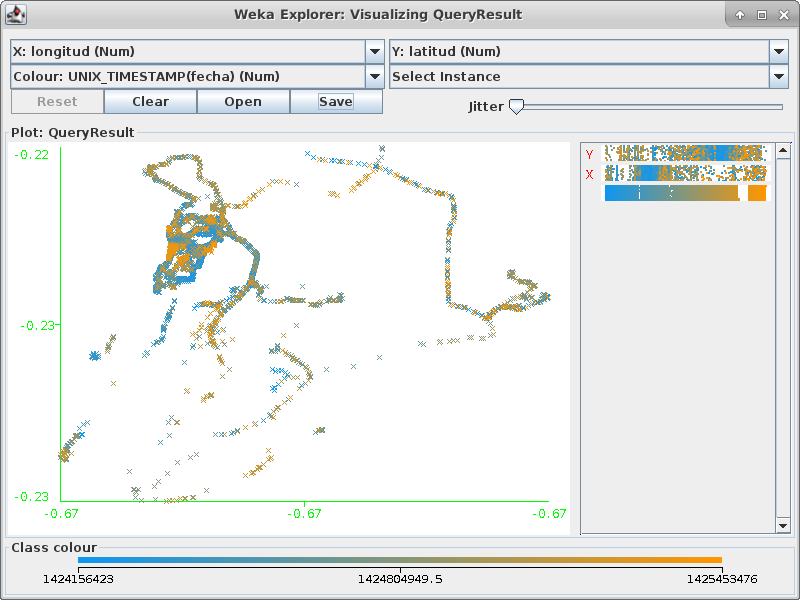
\includegraphics[scale=.5]{wekaImportData.png}
%	\end{center}
%	\caption{Datos asociados al recurso tetra:12082781}
%\end{figure}
%
%Contamos con \textbf{39839} datos para realizar un \textbf{K-means}. El problema de este algoritmo es que hay que especificar el n\'umero de cl\'usters desde un principio, aparte de que los primeros puntos centrales de los cl\'usters se eligen de manera aleatoria. Vamos a realizar una aproximaci\'on de que queremos reducir nuestra base de datos a un $20\%$ por lo que fijaremos unos $8000$ cl\'usters. 
%
%
%\begin{figure}[!htbp]
%	\begin{center}
%	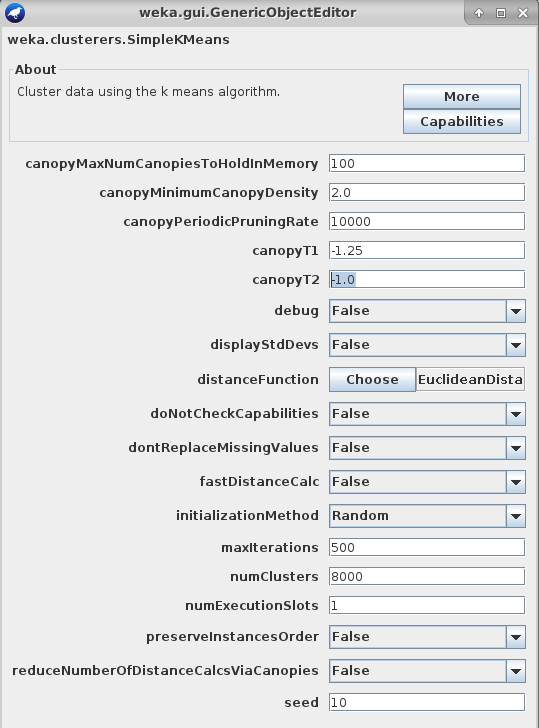
\includegraphics[scale=.5]{wekaKMeansParameters.png}
%	\end{center}
%	\caption{Par\'ametros utilizados a la hora de realizar un K-means}
%\end{figure}
%
%La ejecuci\'on del algoritmo nos devuelve una salida de 8000 cl\'usters, indicando cuantos puntos contiene cada uno y el centro de cada uno de \'estos \ref{App:AppendixE}.
%
%Una mejor visualizaci\'on de los resultados se puede ver aqu\'i, aunque lamentablemente s\'olo respecto a una dimensi\'on (latitud o longitud), en la que podemos obsevar como ha funcionado la asignaci\'on de cada posici\'on a su cl\'uster correspondiente,
%
%\begin{figure}[!htbp]
%	\begin{center}
%	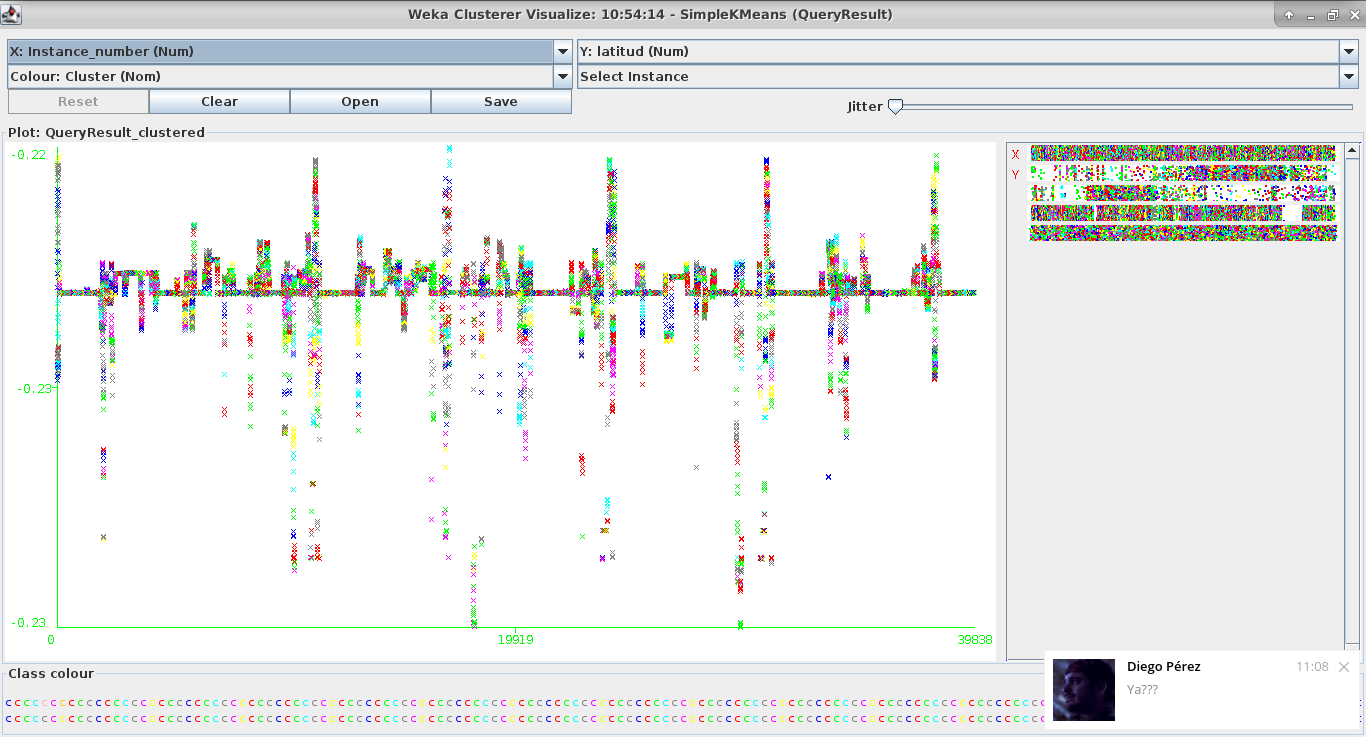
\includegraphics[scale=.4]{wekaKMeansResults.png}
%	\end{center}
%	\caption{Resultados del algoritmo \textbf{K-means}}
%\end{figure}

%%%%%%%%%%%%%%%%%%%%%%%%%%%%%%%%%%%%%%%%%%%%%%%%%%%%%%%%%%%%%%%%%%%%%%%%%%%%%%%%%
%%%%%%%%%%%%%%%%%%%%%%%%%%%%%%%%%%%%%%%%%%%%%%%%%%%%%%%%%%%%%%%%%%%%%%%%%%%%%%%%%

\subsection{DBSCAN}

\textbf{DBSCAN} o \textbf{Density-based spatial clustering of applications with noise} es un algoritmo de \textit{clustering} que dado un conjunto de puntos en un espacio, los agrupa en funci\'on de la densidad de puntos que tengan a su alrededor, dejando a un lado aquellos que tienen una densidad baja. \\

Se considera un conjunto de puntos a aplicar la t\'ecnica. El algoritmo clasificar\'a los puntos en tres grupos, 

\begin{itemize}
	\item Un punto $p$ es considerado \textit{n\'ucleo} si al menos un n\'umero de puntos m\'inimo (al que denotaremos por $minPts$ est\'an a una distancia menor que $\varepsilon$ de $p$. Este conjunto de puntos se considerar\'an \textit{directamente alcanzables} desde $p$.
	\item Un punto $q$ es considerado \textit{alcanzable} de $p$ si existe un camino $p_1, \ldots, p_n$ tal que $p_1=p$ y $p_n=q$, donde cada $p_{i+1}$ es directamente alcanzable desde $p_i$ (todos los puntos del camino son puntos n\'ucleo, excepto quiz\'as $q$).
	\item Todos los puntos que no son considerados ni n\'ucleos ni alcanzables son considerados \textit{aislados}.
\end{itemize}

Ahora, si $p$ es un punto n\'ucleo, entonces forma un cl\'uster con aquellos puntos que sean alcanzables desde $p$. Cada cl\'uster contiene al menos un punto n\'ucleo; y puntos no n\'ucleo pueden formar parte de \'este, pero formaran lo que parten del \textit{borde}, ya que no permiten \textit{alcanzar} m\'as puntos. \\

\begin{figure}[H]\label{fig:DBSCAN}
	\centering
	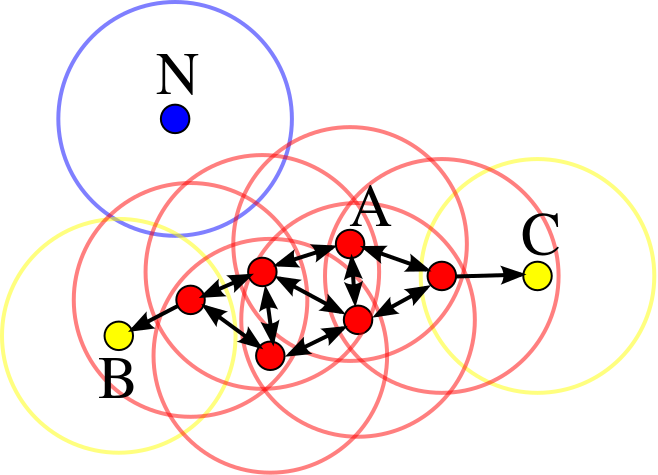
\includegraphics[scale=.5]{DBSCAN.png}
\caption{Diagrama DBSCAN}
\end{figure}

En el diagrama, se puede observar que si fijamos la variable $minPts$ a 3, el punto $A$ y los dem\'as puntos rojos son puntos n\'ucleo, ya que al menos est\'an rodeados de $3$ puntos en su vecindario de radio $\varepsilon$. Como son densamente alcanzables unos con otros, forman un cl\'uster. Los puntos $B$ y $C$ no son puntos n\'ucleo, pero s\'i que son alcanzables desde $A$, por lo que tambi\'en pertenecen al cl\'uster. El punto $N$ es calificiado como aislado o \textit{ruido} ya que no es ni punto n\'ucleo ni densamente alcanzable. \\

La alcanzabilidad no es una relaci\'on sim\'etrica ya que, por definici\'on, ningu\'un punto puede ser alcanzable por un punto no n\'ucleo (un punto no n\'ucleo puede ser alcanzable, pero no puedo \textit{"alcanzar"}). Es necesario definir una noci\'on m\'as fuerte de \textit{conectividad}. Decimos que $p$ y $q$ est\'an densamente conectados si existe un punto $o$ tal que $p$ y $q$ son densamente alcanzables. Esta noci\'on de \textit{densamente conectados} s\'i que es sim\'etrica.\\

Redefinimos la noci\'on de cl\'uster que previamente hab\'iamos definido. Un cl\'uster debe satisfacer dos propiedades:\\

\begin{enumerate}
	\item Todos los puntos deben estar mutuamente \textit{densamente conectados}.
	\item Si un punto $q$ es densamente alcanzable desde un punto $p$ del cl\'uster, $q$ es parte del cl\'uster tambi\'en. 
\end{enumerate}

\textbf{DBSCAN} requiere de dos par\'ametros para empezar: $\varepsilon$ para la noci\'on de vecindario y $minPts$ para el n\'umero m\'inimo de puntos necesario para formar un cl\'uster. Se empieza tomando arbirariamente un punto del conjunto que no haya sido visitado. Se obtiene su vecindario, en el caso de que no exista, este punto se marca como ruido y se pasa al siguiente. Si no es nulo y tiene un n\'umero de puntos mayor que $minPts$, se crea un cl\'uster. \\

Si uno de los puntos del proceso resulta que es parte de un cl\'uster, su vecindario tambi\'en se a\~nade a \'este. Se reitera este proceso, ya que todos los puntos nuevos a\~nadidos del vecindario anterior, son parte del cl\'uster, luego el vecindario de cada uno es a\~nadido. Este proceso se contin\'ua hasta que se obtiene el cl\'uster densamente conectado. \\

\begin{algorithm}[H]\label{DBSCAN}
\begin{algorithmic}[1]
\Function{DBSCAN}{$positions, eps, minPts$}
	\State{C = 0}
	\For{\textbf{each} pos in positions}
		\If{$pos$ has been visited}
			\State{Continue next position}
		\Else
			\State{Mark $pos$ as visited}
			\State{N(pos) = NeighborPts(pos, eps)}
			\If{$length(N(pos)) < MinPts$}
				\State{Mark $pos$ as noise}
			\Else
				\State{C = next Cluster}
				\State{expandCluster(pos, N(pos), C, eps, MinPts)}				
			\EndIf
		
		\EndIf
	\EndFor
\EndFunction
\State{}
\Function{expandCluster}{$P, NeighborPts, C, eps, MinPts$}
	\State{add P to cluster C}
	\For{\textbf{each} P' in NeighborPts}
		\If{P' is not visited}
			\State{Mark P' as visited}
			\State{NeighborPts' = regionQuery(P', eps)}
			\If{$length(NeighborPts') >= MinPts$}
				\State{NeighborPts = NeighborPts joined with NeighborPts'}
			\EndIf
		\EndIf
		\If{P' is not yet member of any cluster}
			\State{add P' to Cluster C}
		\EndIf
	\EndFor
\EndFunction
\State{}
\Function{NeighborPts}{$P, eps$}
	\State{return all points within P's eps-neighborhood (also P)}
\EndFunction
\end{algorithmic}
\caption{\label{alg:DBSCAN} Algoritmo DBSCAN}
\end{algorithm}

\subsubsection{Implementaci\'on en Python}

Se encuentra una implementaci\'on bastante eficaz y sencilla en el repositorio de \href{https://github.com/SushantKafle/DBSCAN}{Sushant Kafle} \ref{dbscanPython}.\\

\begin{python}
from dbscanner import dbscanner
from algorithms.db import connect_db

cur= connect_db("bahia")
recurso = "tetra:12082781"
limit = 1000
cmd = "SELECT latitud, longitud 
	   FROM posicionesgps 
	   WHERE latitud <> 0 and longitud <> 0 
	   AND recurso=\"{0}\" 
	   LIMIT {1};".format(recurso, limit)
cur.execute(cmd)

a=[]
for pos in cur.fetchall():
    a.append([pos[0], pos[1]])

Data = a
eps = 0.0001
MinPts= 5

dbc = dbscanner()
dbc.dbscan(Data, eps, MinPts)
\end{python}

Notar que hemos tomado como valor de $\varepsilon = 0.0001$ ya que es una aproximaci\'on de la distancia media de toma entre posiciones y $5$ es un buen valor a la hora de hacer una consolidaci\'on. El resultado consiste en algunas posiciones marcadas como ruido y $5$ cl\'usters. Debido a que es un proceso muy costoso, nos hemos limitado en este caso a hacer la consolidaci\'on en unas $1000$ posiciones.\\

\begin{figure}[H]
	\begin{center}
	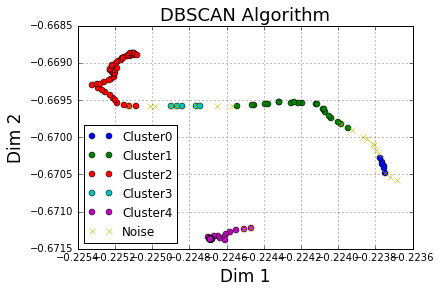
\includegraphics[scale=.7]{dbscan_2_0.png}
	\end{center}
	\caption{Resultados del algoritmo \textbf{DBSCAN} con $\varepsilon = 0.0001$ y $minPts = 5$}
\end{figure}


\subsection{DJ-Cluster}

\textbf{Density-Joinable Cl\'uster}\cite{importantPlaces} es un tipo de algoritmo de \textit{clustering} cuya realizaci\'on depende de la distancia elegida, la cual nos generar\'a un tipo de vecindario en concreto. Este algoritmo localiza puntos significativos sobre el conjunto de todos los puntos, es decir, el centro del cl\'uster. No debemos olvidar que nuestro objetivo es encontrar posiciones significativas en todo nuestro conjunto de posiciones GPS, y \'estos centros de cl\'uster que nos generar\'a este algoritmo nos servir\'an para tal prop\'osito. \\

La idea del algoritmo es la siguiente, para cada punto, calculamos su vecindario. Este vecindario depender\'a de la distancia elegida entre todas las anteriores definidas, y seg\'un cu\'al sea la elegida, depender\'a de una variable $\varepsilon$ o un instante $t_0$ escogido. Se impone la condici\'on de que el n\'umero de puntos conseguido al computar su vecindario sea al menos un \textit{MinPts} definido previamente. Si esta condici\'on no se cumple, se marca la posici\'on actual como \textit{ruido} y se prosigue con la siguiente. En el caso de cumplirse, este nuevo punto es el centro del cl\'uster, junto a su vecindario.  \\

Con este nuevo cl\'uster creado, el siguiente paso es comprobar que este cl\'uster no sea \textit{densamente acoplable} con los que ya llevamos computados. Un cl\'uster es \textit{densamente acoplable} a otro cl\'uster si existe un punto com\'un entre ambos. \\

\begin{figure}[H]
\centering
	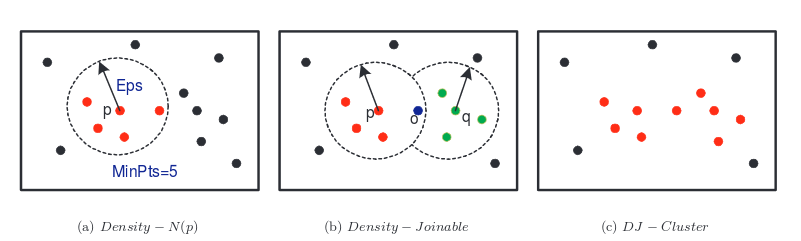
\includegraphics[scale=.7]{djcluster.png}
\caption{DJ-Clustering}
\end{figure}

\begin{algorithm}[!htbp]\label{djCluster}
\begin{algorithmic}[1]
	\For{\textbf{each} $p$ in set $S$}
		\State{Compute neighborhood $N(p)$ for $\varepsilon$ and $MinPts$}
		\If{$N(p)$ is null ($|N(p)| < MinPts$ for $\varepsilon$)}
			\State{Label $p$ as noise}
		\ElsIf{$N(p)$ is density-joinable to an existing cluster} 
			\State{Merge $N(p)$ with the cluster which is density-joinable}
		\Else
			\State{Create a new cluster $C$ based on $N(p)$}
		\EndIf
	\EndFor
\end{algorithmic}
\caption{\label{alg:djcluster} Algoritmo DJ-Cluster}
\end{algorithm}

Durante el proceso, se recorren todos los puntos del conjunto a analizar, calculando cada vecindario de cada punto con un centro $p$ y un radio $\varepsilon$. Si el n\'umero de puntos del vecindario excede esta cantidad m\'inima $MinPts$, entonces es un vecindario a considerar. Este cl\'uster es posteriormente \textit{mergeado} con otros posibles cl\'usters densamente acoplables. \\

Al final de cada iteraci\'on puede ser que el n\'umero de cl\'usters no cambie, porque no existe un nuevo cl\'uster o porque el nuevo cl\'uster sea mergeado con alguno de los ya existentes.\\


El valor de los par\'ametros $\varepsilon$ y $MinPts$ es el que determina el tama\~no de nuestros clusters. En nuestro caso, no buscamos grandes n\'umeros de cl\'usters, sino perder el m\'inimo de informaci\'on posible, por lo que nos convendr\'ia tomar unos valores de $\varepsilon$ y $MinPts$ peque\~nos. \ref{clusteringApproach}

El valor de la variable $\varepsilon$ debe tomarse en funci\'on de la precisi\'on de los aparatos que toman las posiciones.\ref{importantPlaces}. Podemos estimar este par\'amero por unos $20$ metros, que es la precisi\'on de un GPS convencional. \\

Con respecto al valor de $MinPts$, un valor alto de esta par\'ametro implica que los clusters deben ser m\'as densos a la hora de formarse, pero un valor razonable estar\'ia entre $3$ y $10$.\ref{clusteringApproach}.\\

La complejidad de este algoritmo es $\mathcal{O}(n\log{}n)$ \ref{importantPlaces}. \\


%\subsubsection{Estudio con Weka}
%
%Weka tambi\'en permite realizar un \textit{clustering} por DJ-Cluster. Vamos a realizar un primer preprocesado de ratos utilizando la t\'ecnica de \textbf{Canopy}\ref{sec:canoy} que posteriormente est\'a explicada. Como antes, realizaremos primero una consolidaci\'on a unos 8000 cl\'usters y posteriormente aplicaremos \textbf{DJ-Clustering}.\\
%
%Los par\'ametros utilizados en este m\'etodo son los siguientes.\\
%
%\begin{figure}[!htbp]
%\centering
%	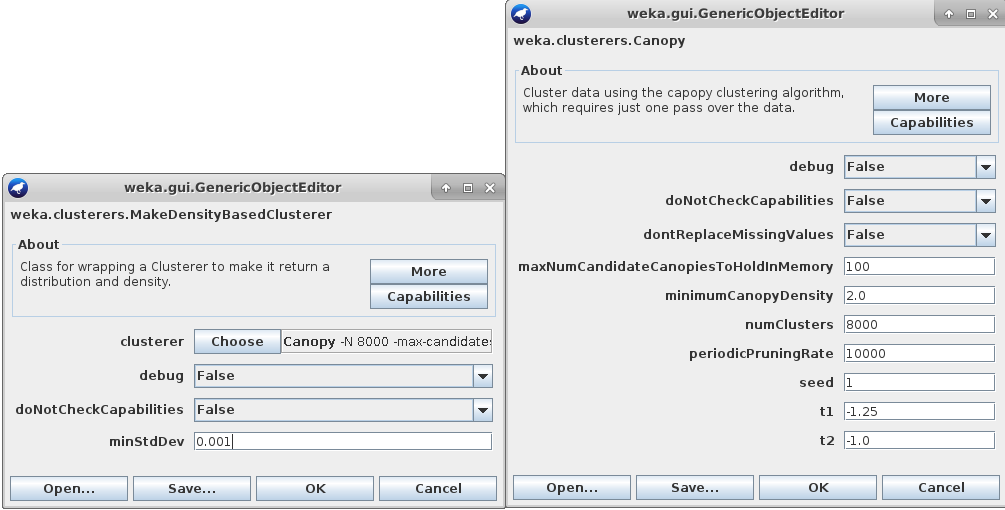
\includegraphics[scale=.55]{wekaDJClusterParametersTotal.png}
%\caption{DJ-Clustering}
%\end{figure}
%
%
%El resultado del \textit{clustering} muestra una primera clasificaci\'on por \textbf{Canopy} en $8000$ posiciones,\\
%
%\begin{verbatim}
%=== Run information ===
%
%Scheme:       weka.clusterers.MakeDensityBasedClusterer -M 0.001 
%													   -W weka.clusterers.Canopy -- 
%													   -N 8000 -max-candidates 100 
%													   -periodic-pruning 10000 
%													   -min-density 2.0 -t2 -1.0 
%													   -t1 -1.25 -S 1
%Relation:     QueryResult
%Instances:    39839
%Attributes:   3
%              latitud
%              longitud
%              UNIX_TIMESTAMP(fecha)
%Test mode:    evaluate on training data
%
%
%=== Clustering model (full training set) ===
%
%MakeDensityBasedClusterer: 
%
%Wrapped clusterer: 
%Canopy clustering
%=================
%
%Number of canopies (cluster centers) found: 8000
%T2 radius: 0,492     
%T1 radius: 0,615     
%
%Cluster 0: -0.224664,-0.67139,1424989490.451634,{28191}
%Cluster 1: -0.224653,-0.671401,1424267875.663668,{10448} 
%Cluster 2: -0.226511,-0.670619,1425045583.497826,{460}
%Cluster 3: -0.225134,-0.66939,1424602410.92381,{210}
%..........................................................
%\end{verbatim}
%
%
%Con la distribuci\'on media de cada par\'ametro a analizar por cl\'uster,\\
%
%\begin{verbatim}
%Fitted estimators (with ML estimates of variance):
%
%Cluster: 0 Prior probability: 0
%
%Attribute: latitud
%Normal Distribution. Mean = 0 StdDev = 1.7976931348623157E308
%Attribute: longitud
%Normal Distribution. Mean = 0 StdDev = 1.7976931348623157E308
%Attribute: UNIX_TIMESTAMP(fecha)
%Normal Distribution. Mean = 0 StdDev = 1.7976931348623157E308
%
%Cluster: 1 Prior probability: 0
%
%Attribute: latitud
%Normal Distribution. Mean = 0 StdDev = 1.7976931348623157E308
%Attribute: longitud
%Normal Distribution. Mean = 0 StdDev = 1.7976931348623157E308
%Attribute: UNIX_TIMESTAMP(fecha)
%Normal Distribution. Mean = 0 StdDev = 1.7976931348623157E308
%
%Cluster: 2 Prior probability: 0
%
%Attribute: latitud
%Normal Distribution. Mean = 0 StdDev = 1.7976931348623157E308
%Attribute: longitud
%Normal Distribution. Mean = 0 StdDev = 1.7976931348623157E308
%Attribute: UNIX_TIMESTAMP(fecha)
%Normal Distribution. Mean = 0 StdDev = 1.7976931348623157E308
%
%Cluster: 3 Prior probability: 0
%
%Attribute: latitud
%Normal Distribution. Mean = -0.2252 StdDev = 0.001
%Attribute: longitud
%Normal Distribution. Mean = -0.6695 StdDev = 0.001
%Attribute: UNIX_TIMESTAMP(fecha)
%Normal Distribution. Mean = 1424636974 StdDev = 411992.8182
%
%\end{verbatim}
%
%Y m\'as adelante visualizamos el \textit{clustering} por DJ-Cluster, en la que podemos observar que se ha realizado una consolidaci\'on m\'as fina.
%
%\begin{verbatim}
%Time taken to build model (full training data) : 105.91 seconds
%
%=== Model and evaluation on training set ===
%
%Clustered Instances
%
%   9          9 (  0%)
%  10          2 (  0%)
%  12          3 (  0%)
%  13          3 (  0%)
%  --------------------
%\end{verbatim}
%
%Mostramos s\'olamente las primeras instancias, ya que son muchos cl\'usters, pero se observa que los 8 primeros han sido eliminados al igual que el n\'umero 11.


%%%%%%%%%%%%%%%%%%%%%%%%%%%%%%%%%%%%%%%%%%%%%%%%%%%%%%%%%%%%%%%%%%%%%%%%%%%%%%%%%%%%%%%%%%%%%%%
%%%%%%%%%%%%%%%%%%%%%%%%%%%%%%%%%%%%%%%%%%%%%%%%%%%%%%%%%%%%%%%%%%%%%%%%%%%%%%%%%%%%%%%%%%%%%%%
%%%%%%%%%%%%%%%%%%%%%%%%%%%%%%%%%%%%%%%%%%%%%%%%%%%%%%%%%%%%%%%%%%%%%%%%%%%%%%%%%%%%%%%%%%%%%%%
%%%%%%%%%%%%%%%%%%%%%%%%%%%%%%%%%%%%%%%%%%%%%%%%%%%%%%%%%%%%%%%%%%%%%%%%%%%%%%%%%%%%%%%%%%%%%%%

\pagebreak
\section{Comparativa de resultados}

Vamos a realizar un estudio de los m\'etodos estudiados para dos sujetos en concreto. De dos sujetos de nuestra base de datos, tomaremos 2.000 posiciones y veremos c\'omo responden a cada uno de los algoritmos. A la hora de importar los datos a Weka, aplicamos un filtro de Normalizaci\'on, dado que un futuro vamos a estar utilizando la distancia eucl\'idea en nuestros algoritmos, debemos normalizar los datos para que ninguno de estos pese sobre los dem\'as. Como la fecha est\'a representada por un \texttt{timestamp}, \'este tendr\'ia much\'isimo m\'as valor a la hora de realizar la consolidaci\'on.

\begin{figure}[H]
	\begin{tabular}{| l | l |}
	\hline
		Sujeto 1 & tetra:12082781 \\
		Sujeto 2 & tetra:12082364 \\	
	\hline
	\end{tabular}
\end{figure}

Se puede visualizar a simple vista que los datos son algo dispares entre s\'i, es decir, estamos cogiendo dos sujetos que no siguen con distintos patrones de movimiento. \\

\begin{figure}[H]
	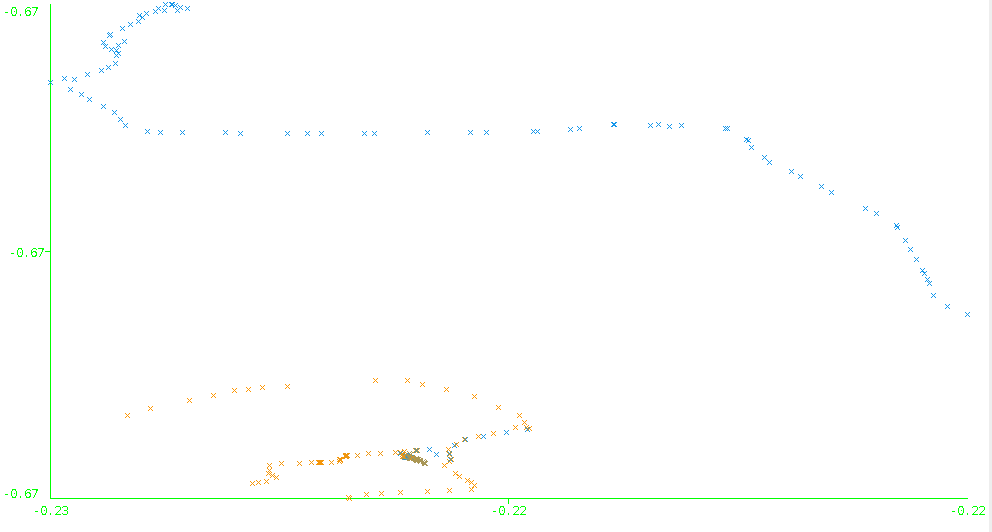
\includegraphics[scale=.5]{../comparativa/sujeto1.png}
	\caption{Distribuci\'on de las 2.000 posiciones del Sujeto 1}
\end{figure}

\begin{figure}[H]
	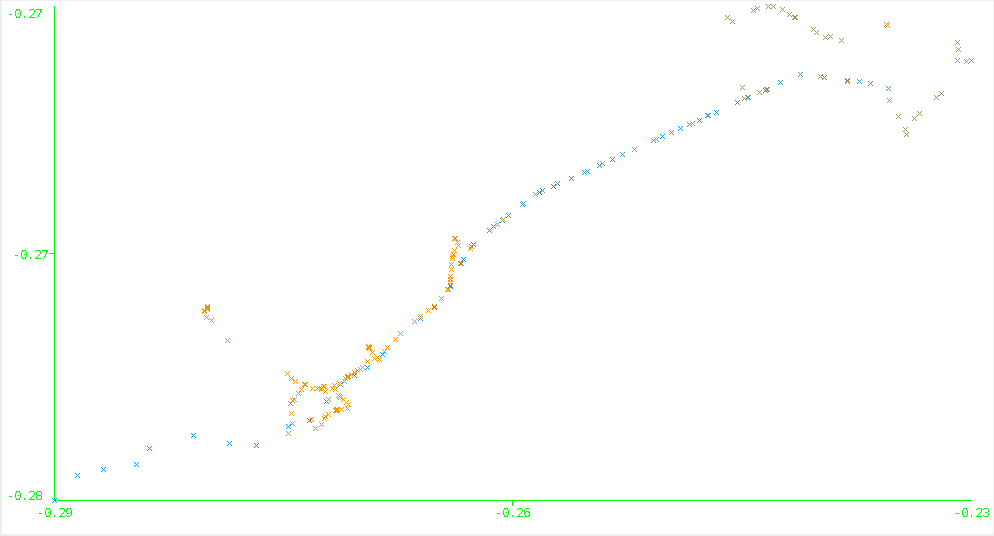
\includegraphics[scale=.5]{../comparativa/sujeto2.png}
	\caption{Distribuci\'on de las 2.000 posiciones del Sujeto 2}
\end{figure}


\subsection{Resultados con K-means}

Vamos a realizar un estudio \textbf{K-means} para ambos sujetos con los mismos par\'ametros que previamente hab\'iamos aplicado, pero en vez de realizar una consolidaci\'on al $20\%$, vamos a reducir el n\'umero de posiciones a $500$, es decir, una consolidaci\'on al $25\%$. 

\subsubsection{Sujeto 1}

\begin{verbatim}
kMeans
======

Number of iterations: 10
Within cluster sum of squared errors: 0.15548219897667379

Initial starting points (random):

Cluster 0: 3299150891,tetra:12082781,-0.224687,-0.67137,1424176713
Cluster 1: 3299151121,tetra:12082781,-0.224684,-0.671368,1424176748
Cluster 2: 3299184432,tetra:12082781,-0.224685,-0.671368,1424183306
Cluster 3: 3299175108,tetra:12082781,-0.224682,-0.671373,1424181474
Cluster 4: 3299044269,tetra:12082781,-0.225253,-0.669394,1424156873
...
\end{verbatim}

Se han realizado $10$ iteraciones y se ha llegado a un error cuadr\'atico de $0.15$. Observando el n\'umero de posiciones que ha agrupado por cl\'uster, podemos observar que var\'ian entre $1$ y $9$, lo cual es una buena media, ya que no ha agrupado demasiadas posiciones en un mismo cl\'uster. \\ 

Se puede observar mejor en la gr\'afica. Cada cl\'uster est\'a representado por un color distinto. En la parte superior de esta gr\'afica, podemos observar que ha seguido un camino con respecto al tiempo en una direcci\'on, mientras que en la parte superior ha pasado varias veces por un mismo sitio, y aparece una aglomeraci\'on de colores en un punto. Esto se debe a que para nuestro estudio hemos introducido tambi\'en la variable temporal, por lo que no puede agrupar todas esas posiciones en un mismo cl\'uster, ya que no lo est\'an, debido a que vienen de varios instantes distintos. \\

\begin{figure}[H]
	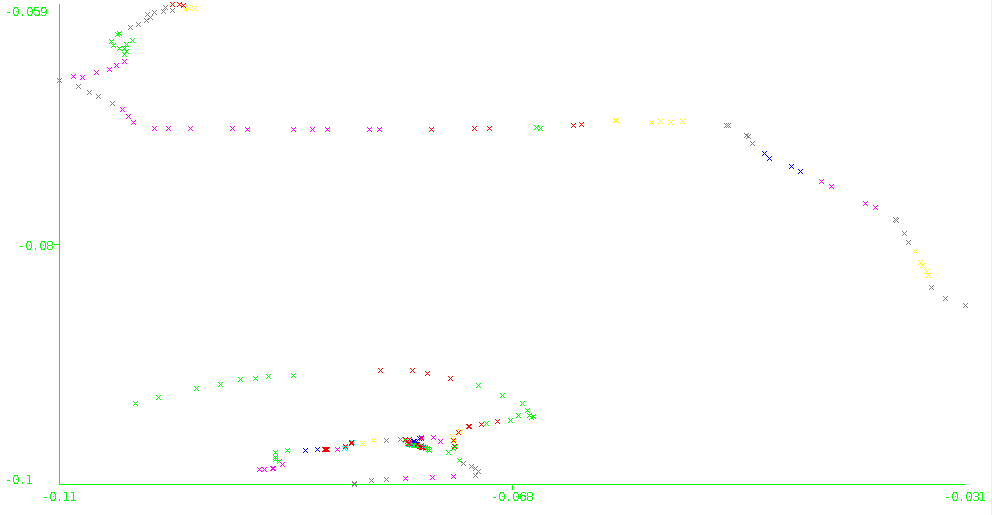
\includegraphics[scale=.5]{../comparativa/kMeansSujeto1.png}
	\caption{Estudio K-means para el Sujeto 1}
\end{figure}


\subsubsection{Sujeto 2}

Realizamos el mismo estudio con el Sujeto 2,\\

\begin{verse}
=== Model and evaluation on training set ===

Clustered Instances

  0        10 (  1%)
  1         1 (  0%)
  2        33 (  2%)
  3        16 (  1%)
  4         4 (  0%)
  5        33 (  2%)
  6        20 (  1%)
  7        14 (  1%)
  8        11 (  1%)
  9        26 (  1%)
 10         1 (  0%)
 ...
 489         2 (  0%)
490         1 (  0%)
491         2 (  0%)
492         1 (  0%)
493         1 (  0%)
494         1 (  0%)
495         1 (  0%)
496         1 (  0%)
497         2 (  0%)
498         2 (  0%)
499         2 (  0%)
\end{verse}

Se observa que en este caso la asignaci\'on de cl\'usters es a\'un m\'as dispar que en el sujeto 1, ya que se asignan muchas posiciones para los primeros cl\'usters dejando para los del final casi ninguna (dado que le hemos fijado un resultado final de $500$ cl\'usters). En este sentido, se puede observar que las primeras posiciones (en un contexto temporal) se asignan bien a los cl\'usters, pero esta limitaci\'on de tener que asignar un valor al n\'umero de cl\'usters que deseamos obtener, es la que echa a perder el m\'etodo. Esto que en un principio no deber\'ia ser malo porque nos asegurar\'ia la reducci\'on de espacio en disco que buscamos es la que en el sujeto 2, nos arruina el resultado. Visualmente, las primeras posiciones se encuentran en la franja de abajo a la izquierda, mientras que las finales son las de la franja de arriba a la izquierda. \\

\begin{figure}[H]
	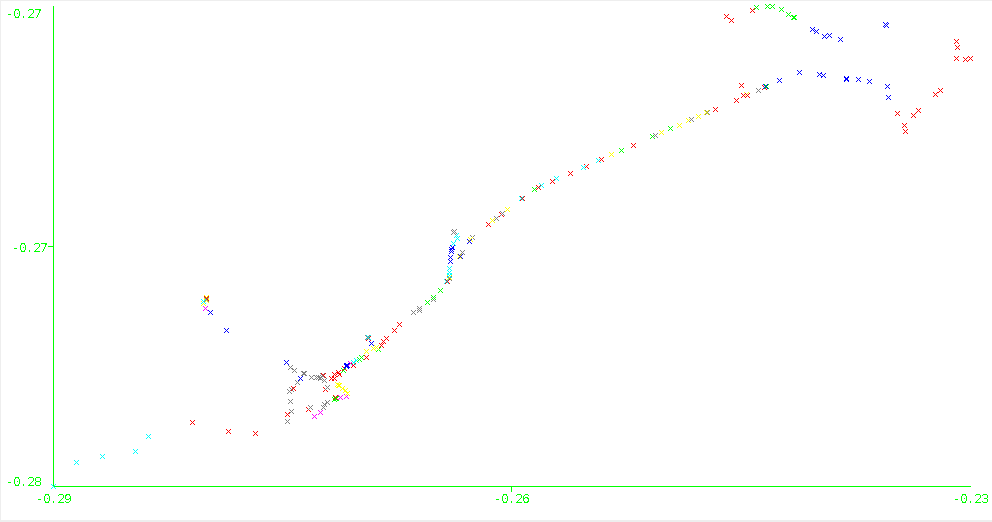
\includegraphics[scale=.5]{../comparativa/kMeansSujeto2.png}
	\caption{Estudio K-means para el Sujeto 1}
\end{figure}

\subsection{Resultados con DBSCAN}

Utilizaremos los mismos par\'ametros utilizados para el m\'etodo \textbf{DBSCAN} previamente estudiado, un valor de $\varepsilon = 0.0001$ y un valor de $minPts = 5$. Tomaremos $1000$ datos de cada sujeto y los compararemos,\\

\subsubsection{Sujeto 1}

\begin{python}
cur= connect_db("bahia")
recurso = "tetra:12082781"
limit = 2000
cmd = "SELECT latitud, longitud 
		FROM posicionesgps 
		WHERE latitud <> 0 and longitud <> 0 and recurso=\"{0}\" 
		LIMIT {1};".format(recurso, limit)
cur.execute(cmd)

a=[]
for pos in cur.fetchall():
    a.append([pos[0], pos[1]])

Data = a
eps = 0.0001
MinPts=5

dbc = dbscanner()
dbc.dbscan(Data, eps, MinPts)
\end{python}

\begin{figure}[H]
	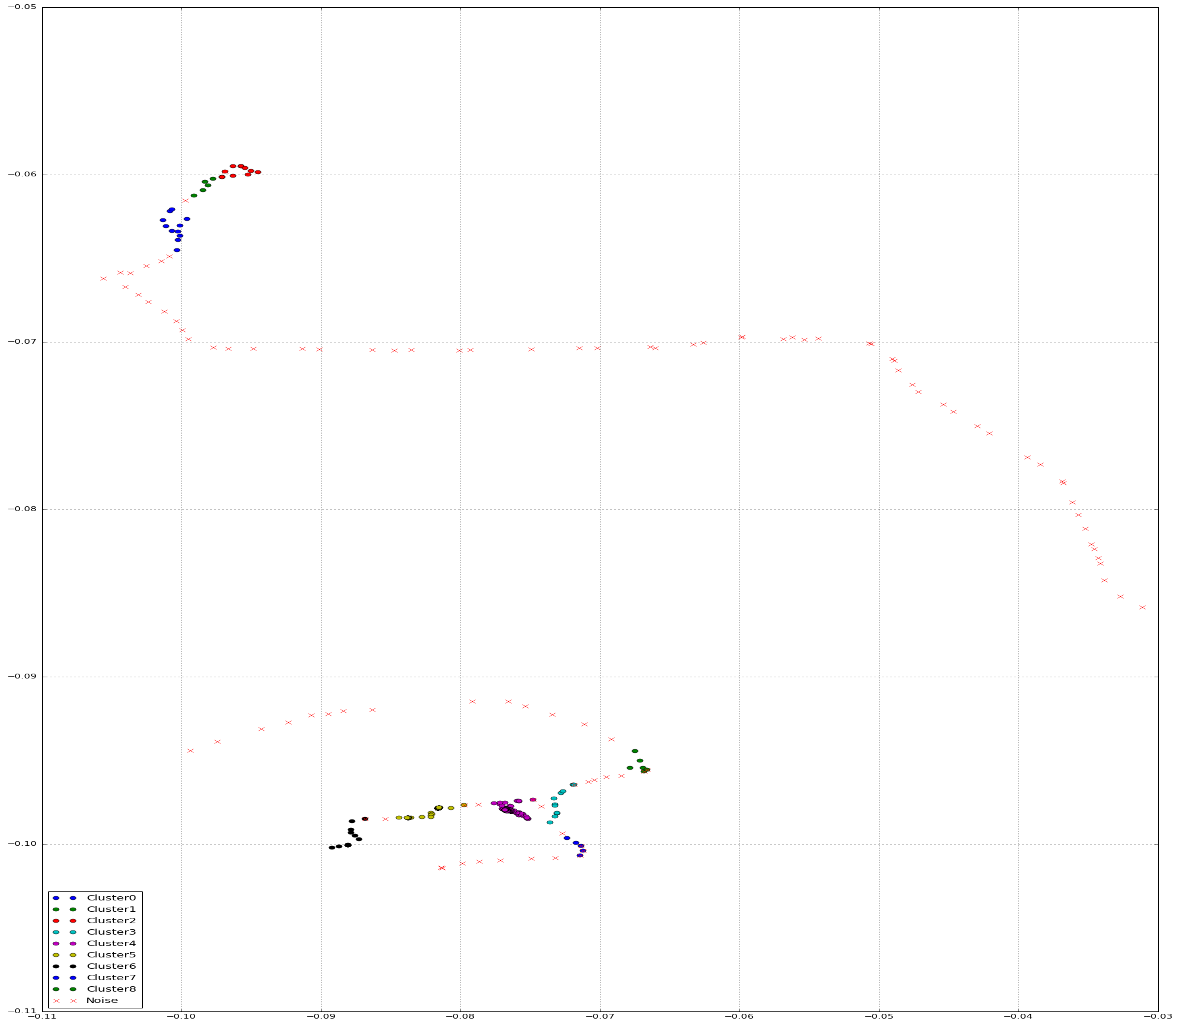
\includegraphics[scale=.7]{../comparativa/dbscanSujeto1.png}
	\caption{Estudio DBSCAN para el Sujeto 1}
\end{figure}

Una de las cosas positivas que se puede decir del algoritmo \textbf{DBSCAN} es que identifica puntos como \textit{ruido}, cosa que los algoritmos de \textbf{K-means} y \textbf{DJ-Cluster} no hacen, ya que asignan simplemente esos puntos a un cl\'uster de un \'unico punto.\\

\subsubsection{Sujeto 2}

\begin{python}
cur= connect_db("bahia")
recurso = "tetra:12082781"
limit = 2000
cmd = "SELECT latitud, longitud 
		FROM posicionesgps 
		WHERE latitud <> 0 and longitud <> 0 and recurso=\"{0}\" 
		LIMIT {1};".format(recurso, limit)
cur.execute(cmd)

a=[]
for pos in cur.fetchall():
    a.append([pos[0], pos[1]])

Data = a
eps = 0.0001
MinPts=5

dbc = dbscanner()
dbc.dbscan(Data, eps, MinPts)
\end{python}

\begin{figure}[H]
	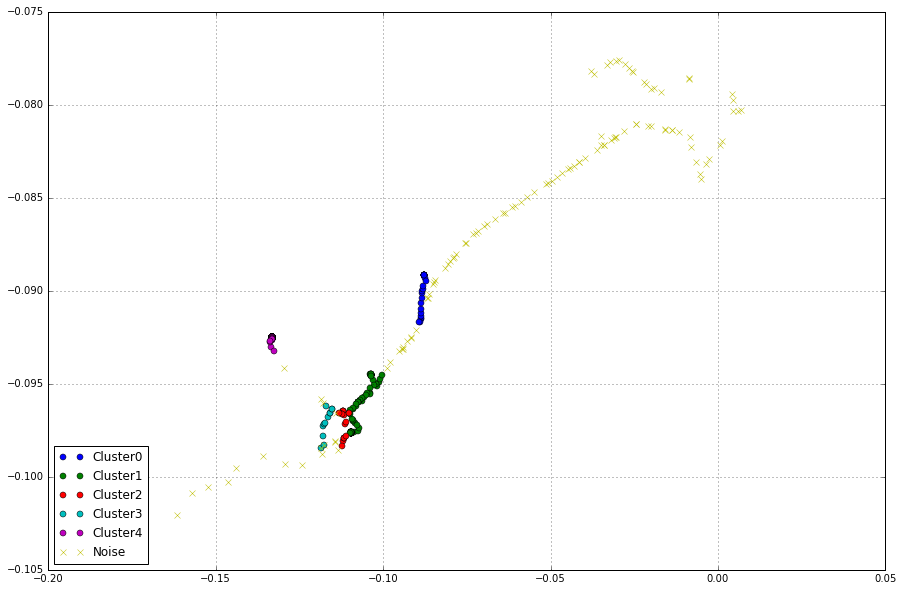
\includegraphics[scale=.7]{../comparativa/dbscanSujeto2.png}
	\caption{Estudio DBSCAN para el Sujeto 2}
\end{figure}

Otro de los problemas encontrados a la hora de utilizar el algoritmo \textbf{DBSCAN} es que la implementaci\'on utilizada s\'olo involucra las variables latitud y longitud, por lo que la consolidaci\'on no tendr\'a en cuenta si un sujeto pasa repetidas veces por un mismo lugar.\\

\subsection{Resultados con DJ-Cluster}

Realizaremos un estudio \textbf{DJ-Cluster} utilizando un preprocesado de datos \textbf{Canopy} fijando una desviaci\'on m\'inima est\'andar de $0.001$. \\

\subsubsection{Sujeto 1}

Si en el preprocesado de \textbf{Canopy} no especificamos el n\'umero de cl\'usters que queremos conseguir, \'este consolida demasiados datos d\'andonos un resultado de s\'olamente $4$ cl\'usters, lo cual no nos es interesante, ya que se pierde demasiada informaci\'on. \\

Fijaremos pues la variable del n\'umero de cl\'usters en los $500$ que previamente hemos elegido,\\


\begin{verbatim}
=== Run information ===

Scheme:       weka.clusterers.MakeDensityBasedClusterer 
					-M 0.001 -W weka.clusterers.Canopy -- 
					-N 500 -max-candidates 100 -periodic-pruning 10000 
					-min-density 2.0 -t2 -0.001 -t1 -0.001 
					-S 1 
Relation:     QueryResult
Instances:    2000
Attributes:   5
              latitud
              longitud
              UNIX_TIMESTAMP(fecha)
Ignored:
              id
              recurso
Test mode:    evaluate on training data


=== Clustering model (full training set) ===

MakeDensityBasedClusterer: 

Wrapped clusterer: 
Canopy clustering
=================

Number of canopies (cluster centers) found: 500
T2 radius: 0,504     
T1 radius: 0,001     

Cluster 0: -0.225087,-0.669237,1424157165.818182,{55} <0>
Cluster 1: -0.224685,-0.671368,1424171523.408413,{1474} <1>
Cluster 2: -0.224713,-0.671363,1424188821.625571,{438} <2>
Cluster 3: -0.223987,-0.669914,1424157151.060606,{33} <3>
....

Clustered Instances
....
 12        14 (  1%)
 13         2 (  0%)
 14         2 (  0%)
 15         2 (  0%)
 18         3 (  0%)
 19         5 (  0%)
 20         4 (  0%)
....
\end{verbatim} 

A\'un a pesar del preprocesado por \textit{canopies}, vemos que la asignaci\'on de las posiciones a los cl\'usters ha sido menos suave, ya que podemos encontrarnos gran cantidad de cl\'usters con m\'as de $10$ posiciones agrupadas y bastantes con s\'olo $2$. Sin embargo, visualmente, \\

\begin{figure}[H]
	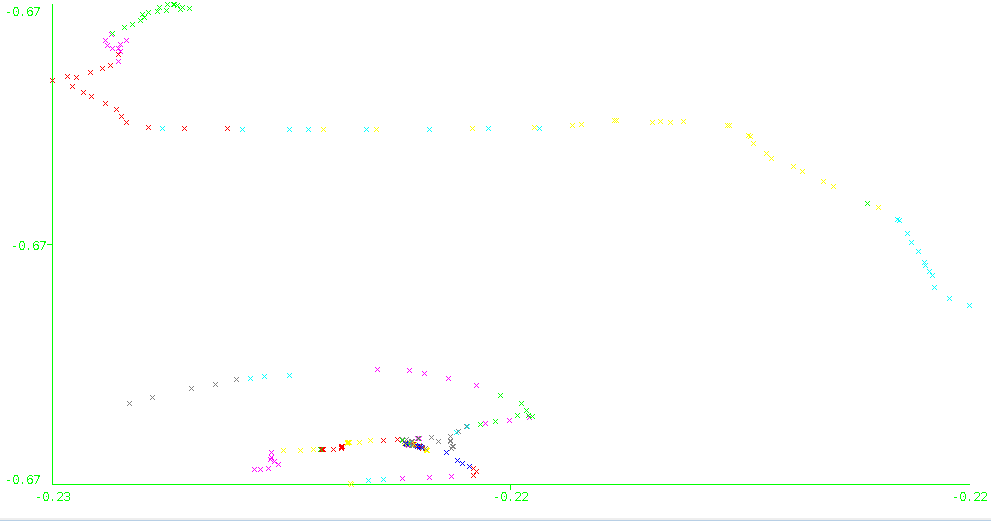
\includegraphics[scale=.5]{../comparativa/djClusterSujeto1.png}
	\caption{Estudio Dj-Cluster para el Sujeto 1}
\end{figure}

Podemos observar que la parte de abajo del conglomerado que K-means no llegaba a resolver, DJ-Cluster hace una mejor selecci\'on de cl\'usters en esta zona. \\

\subsubsection{Sujeto 2}

En el sujeto dos podemos pensar que DJ-Cluster tambi\'en peca de demasiada clusterizaci\'on a\'un a pesar de que hemos indicado que en el preprocesado \textbf{Canopy} utilice $500$ cl\'usters.\\

\begin{verbatim}
=== Model and evaluation on training set ===

Clustered Instances

 14         4 (  0%)
 38         8 (  0%)
 42      1536 ( 77%)
\end{verbatim}

Pero, si observamos el cl\'uster n\'umero $42$,\\

\begin{verbatim}
Cluster: 42 Prior probability: 0.0244

Attribute: latitud
Normal Distribution. Mean = -0.2211 StdDev = 0.002
Attribute: longitud
Normal Distribution. Mean = -0.6726 StdDev = 0.0008
Attribute: fecha
Normal Distribution. Mean = 2015 StdDev = 0
\end{verbatim}

Vemos que la probabilidad de que una posici\'on caiga en este cl\'uster es de $0.02\%$. Haciendo unas sencillas consultas en MySQL sobre la regi\'on fuertemente consolidada y la regi\'on final en la que vemos que no ha habido tanta consolidaci\'on,

\begin{lstlisting}[language=sql, columns=fullflexible, basicstyle=\small, frame=tbrl, showstringspaces=false]
mysql> SELECT id, latitud, longitud 
	   FROM posicionesgps 
	   WHERE recurso = 'tetra:12086044' 
	   LIMIT 130, 5;
\end{lstlisting}

\begin{figure}[H]
	\begin{tabular}{| l | l | l |}
	\hline
	\rowcolor{LightCyan}
	\hline
  		id & latitud & longitud \\
	\hline
		3299639690 & -0.22662244737148285 & -0.6721994876861572 \\
		3299639777 & -0.22662168741226196 & -0.6722030639648438 \\
		3299639884 & -0.22662168741226196 & -0.6722030639648438 \\
		3299639985 & -0.22662225365638733 & -0.6721988916397095 \\
		3299640070 & -0.22662188112735748 & -0.6722032427787781 \\
	\hline
	\end{tabular}
	\caption{Consulta SQL de los resultados fuertemente consolidados}
\end{figure}


\begin{lstlisting}[language=sql, columns=fullflexible, basicstyle=\small, frame=tbrl, showstringspaces=false]
mysql> SELECT id, latitud, longitud 
	   FROM posicionesgps 
	   WHERE recurso = 'tetra:12086044' 
	   LIMIT 1990, 5;
\end{lstlisting}

\begin{figure}[H]
	\begin{tabular}{| l | l | l |}
	\hline
	\rowcolor{LightCyan}
	\hline
  		id & latitud & longitud \\
	\hline
	3299801551 & -0.2217489778995514 & -0.6714484095573425 \\
	3299801554 & -0.22178474068641663 & -0.6714062690734863 \\
	3299801901 & -0.22180871665477753 & -0.6713294982910156 \\
	3299801938 & -0.2218199521303177 & -0.671276867389679 \\
	3299802276 & -0.2218736857175827 & -0.6711682677268982 \\
	\hline
	\end{tabular}
	\caption{Consulta SQL de los resultados fuertemente consolidados}
\end{figure}

Se puede observar que en la primera tabla, las posiciones no han variado mucho, ya que s\'olo se observa variaci\'on a partir del sexto decimal, sin embargo, en la segunda tabla la variaci\'on de la posici\'on es mucho mayor, ya que la empiezan a cambiar a partir del cuarto. Esto representa un mayor movimiento del sujeto, por lo que podemos concluir que \textbf{DJ-Cluster} ha realizado una buena consolidaci\'on.


\pagebreak
\section{Notas y conclusiones}

Entre estos m\'etodos tambi\'en ha sido valorado el estudiar m\'etodos de \textit{clustering} jerarquizados. Sin embargo, la idea principal que desech\'o el estudio de \'estos fue que la complejidad de un \textit{clustering} aglomerativo jerarquizado es de $\mathcal{O}(n^3)$ y la de \textit{clustering} divisivo tambi\'en jerarquizado es de $\mathcal{O}(2^n)$. \\


\pagebreak
\section{Herramientas utilizadas}

\begin{enumerate}
	\item \textbf{Weka} (Waikato Environment for Knowledge Analysis, en espa\~nol «entorno para an\'alisis del conocimiento de la Universidad de Waikato») es una plataforma de software para el aprendizaje autom\'atico y la miner\'ia de datos escrito en Java y desarrollado en la Universidad de Waikato. Weka es software libre distribuido bajo la licencia GNU-GPL.\ref{weka}
	
	\item \textbf{Python} se trata de un lenguaje de programaci\'on multiparadigma, ya que soporta orientaci\'on a objetos, programaci\'on imperativa y, en menor medida, programaci\'on funcional. Es un lenguaje interpretado, usa tipado dinámico y es multiplataforma.
	
	\item \textbf{R} es un lenguaje y entorno de programaci\'on para an\'alisis estad\'istico y gr\'afico. \textbf{R} se distribuye bajo la licencia GNU GPL y est\'a disponible para los sistemas operativos Windows, Macintosh, Unix y GNU/Linux.\ref{r}
	
	\item \textbf{GitHub} es una plataforma de desarrollo colaborativo para alojar proyectos utilizando el sistema de control de versiones Git.
	
	\item \textbf{MySQL} es un sistema de gesti\'on de bases de datos relacional, multihilo y multiusuario bajo una licencia GNU GPL para uso no comercial.
	
\end{enumerate}


\newpage


\appendix
\section{Impementaci\'on de consolidaci\'on por distancia} \label{App:AppendixA}

\begin{python}
"Consolidation By distance"
def ConsolidationByDistance(listPositions, typeOfDistance, eps, t0):
	i = 0
	result = []
	while i < len(listPositions) - 1:
		# Neighborhood: Distance EU simple
		if typeOfDistance == 0:
			if not listPositions[i].is_in_neighborhoodByEUSimple(listPositions[i+1], eps):
				result.append(listPositions[i])
		# Neighborhood: Distance EU relative to speed
		elif typeOfDistance == 1:
			if not listPositions[i].is_in_neighborhoodByEURelativeSpeed(listPositions[i+1], eps):
				result.append(listPositions[i])
		# Neighborhood t0 reachable
		elif typeOfDistance == 2:
			if not listPositions[i].is_in_neighborhoodT0Reachable(listPositions[i+1], t0):
				result.append(listPositions[i])
		else:
			raise ValueError('That distance does not exist')

		i=i+1

	result.append(listPositions[len(listPositions) - 1])

	return result

\end{python}

\newpage
\section{Impementaci\'on de consolidaci\'on por adelgazamiento} \label{App:AppendixB}

\begin{python}
"Consolidation by thinning."
def ConsolidationByThinning(listPositions, k, j):
	if k >= j:
		raise ValueError('K tiene que ser menor que J')
        
	i = 0
	result = []
	while i < len(listPositions) - 1:
		if i%j == 0:
			l = 0
			while l < k:
				result.append(listPositions[i - l])
				l = l+1
			i = i+1

	return result
\end{python}


\newpage
\section{Impementaci\'on de DJ-Cluster} \label{App:AppendixC}

\begin{python}
from position import Position, Cluster

"Dj-Clustering Algorithm"
def DjCluster(setPoints, typeDistance, eps, minPoints, t0):

	listClusters = []
	listNoises = []

	for p in setPoints:
		np = computeNeighborhood(p, setPoints, typeDistance, minPoints, eps, t0)

		if np is None:
			listNoises.append(p) 
		else:
			result = np.isDensityJoinable(listClusters)

			if result is None:
				listClusters.append(np) 
			else:
				result.mergeCluster(np)

	return [listClusters, listNoises]

"Compute Neighborhood"
def computeNeighborhood(p, setPoints, typeDistance, minPoints, eps, t0):
	pointsOfCluster = []
	for q in setPoints:
		if typeDistance == 0:
			if p.is_in_neighborhoodByEUSimple(q, eps):
				pointsOfCluster.append(q)
		elif typeDistance == 1:
			if p.is_in_neighborhoodEURelativeSpeed(q, eps):
				pointsOfCluster.append(q)
		elif typeDistance == 2:
			if p.is_in_neighborhoodT0Reachable(q, t0):
				pointsOfCluster.append(q)

	if len(pointsOfCluster) < minPoints:
		return None
	else:
		return Cluster(p, pointsOfCluster)			

\end{python}

\newpage
\section{Impementaci\'on de Canopy} \label{App:AppendixD}

\begin{python}
from sklearn.metrics.pairwise import pairwise_distances
import numpy as np

# T1 > T2 for overlapping clusters
# T1 = Distance to centroid point to not include in other clusters
# T2 = Distance to centroid point to include in cluster
# T1 > T2 for overlapping clusters
# T1 < T2 will have points which reside in no clusters
# T1 == T2 will cause all points to reside in mutually exclusive clusters

def canopy(X, T1, T2, distance_metric='euclidean', filemap=None):
    canopies = dict()
    X1_dist = pairwise_distances(X, metric=distance_metric)
    canopy_points = set(range(X.shape[0]))
    while canopy_points:
        point = canopy_points.pop()
        i = len(canopies)
        canopies[i] = {"c":point, "points": list(np.where(X1_dist[point] < T2)[0])}
        canopy_points = canopy_points.difference(set(np.where(X1_dist[point] < T1)[0]))
    if filemap:
        for canopy_id in canopies.keys():
            canopy = canopies.pop(canopy_id)
            canopy2 = {"c":filemap[canopy['c']], "points":list()}
            for point in canopy['points']:
                canopy2["points"].append(filemap[point])
            canopies[canopy_id] = canopy2
    return canopies

\end{python}

\newpage
\section{Impementaci\'on de consolidaci\'on por tiempo} \label{App:AppendixF}

\begin{python}
"Consolidation by time. Deletes positions too close by time."
def ConsolidationByTime(listPositions, lapse):
	i = 0
	result = []
	while i < len(listPositions) - 1:
		if not listPositions[i].is_neighboorhoudByTime(listPositions[i+1], lapse):
			result.append(listPositions[i])
		i=i+1
	#Por defecto anadiremos la ultima posicion, ya que no tiene siguiente con quien comparar
	result.append(listPositions[len(listPositions) - 1])

	return result
\end{python}


\newpage
\section{Resulados Algoritmo K-means utilizando Weka} \label{App:AppendixE}

\begin{verbatim}

=== Run information ===

Scheme:       weka.clusterers.SimpleKMeans -init 0 -max-candidates 100 
										  -periodic-pruning 10000 
										  -min-density 2.0 -t1 -1.25 
										  -t2 -1.0 -N 8000 
										  -A "weka.core.EuclideanDistance 
										  -R first-last" -I 500 
										  -num-slots 1 -S 10
Relation:     QueryResult
Instances:    39839
Attributes:   3
              latitud
              longitud
              UNIX_TIMESTAMP(fecha)
Test mode:    evaluate on training data


=== Clustering model (full training set) ===


kMeans
======

Number of iterations: 19
Within cluster sum of squared errors: 0.6346425074677955

Initial starting points (random):

Cluster 0: -0.224685,-0.671374,1424274995
Cluster 1: -0.224541,-0.671549,1424233683
Cluster 2: -0.224685,-0.671371,1424506207
Cluster 3: -0.224684,-0.671368,1424533080
Cluster 4: -0.224685,-0.67137,1424937795
Cluster 5: -0.225005,-0.671538,1425054445
Cluster 6: -0.224681,-0.671371,1425364201
Cluster 7: -0.224511,-0.671435,1424547762
Cluster 8: -0.224685,-0.671372,1425445944
Cluster 9: -0.224512,-0.67143,1424593627
Cluster 10: -0.224688,-0.671369,1424801082
Cluster 11: -0.224542,-0.671549,1424212221
Cluster 12: -0.224685,-0.671368,1424177841
Cluster 13: -0.224686,-0.67137,1425101454
Cluster 14: -0.224681,-0.671372,1424250539
Cluster 15: -0.224685,-0.67137,1424250305
............................................

Time taken to build model (full training data) : 240.83 seconds

=== Model and evaluation on training set ===

Clustered Instances

   0          3 (  0%)
   1          2 (  0%)
   2          1 (  0%)
   3          3 (  0%)
   4          4 (  0%)
   5          4 (  0%)
   6          4 (  0%)
   7          2 (  0%)
   8          2 (  0%)
   9          5 (  0%)
  10          3 (  0%)
  11          3 (  0%)
  12          7 (  0%)
  13          6 (  0%)
  14         13 (  0%)
  15         13 (  0%)
............................................

\end{verbatim}

%%%%%%%%%%%%%%%%%%%%%%%%%%%%%%%%%%%%%%%%%%%%%%%%%%%%%%%%%%%%%%%%%%%%%%%%%%%%%%%%%%%%%%%%%%%%%%%%
%%%%%%%%%%%%%%%%%%%%%%%%%%%%%%%%%%%%%%%%%%%%%%%%%%%%%%%%%%%%%%%%%%%%%%%%%%%%%%%%%%%%%%%%%%%%%%%%
%%%%%%%%%%%%%%%%%%%%%%%%%%%%%%%%%%%%%%%%%%%%%%%%%%%%%%%%%%%%%%%%%%%%%%%%%%%%%%%%%%%%%%%%%%%%%%%%


\newpage

\addcontentsline{toc}{section}{Bibliograf\'ia}
\begin{thebibliography}{50}


\bibitem{lifePatter}\label{lifePatter} Yang Ye, Yu Zheng, Yukun Chen, Jianhua Feng, Xing Xie
\\ \href{http://citeseerx.ist.psu.edu/viewdoc/download?doi=10.1.1.361.9085&rep=rep1&type=pdf}{\textit{Mining Individual Life Pattern Based on Location History}}

\bibitem{importantPlaces}\label{importantPlaces} Changqing Zhou, Nupur Bhatnagar, Shashi Shekhar, Loren Terveen
\\ \href{http://www-users.cs.umn.edu/~czhou/pub/place-important_v3.pdf}{\textit{Mining Personally Important Places from GPS Track}} 

\bibitem{clusteringApproach}\label{clusteringApproach} Changqing Zhou, Dan Frankowski, Pamela Ludford, Shashi Shekhar, Loren Terveen
\\ \href{http://files.grouplens.org/papers/zhou-acmgis04.pdf}{\textit{Discovering Personal Gazetteers: An Interactive Clustering Approach}}

\bibitem{canopy}\label{canopy} Andrew McCallum, Kamal Nigam, Lyle H. Ungar \\
\href{http://www.kamalnigam.com/papers/canopy-kdd00.pdf}{\textit{Efficient Clustering of High-Dimensional Data Sets with Application to Reference Matching}}

\bibitem{canopyGitHub} \label{canopyGitHub} \href{https://github.com/gdbassett}{\textit{Gabe}}'s Gist \\ 
\href{https://gist.github.com/gdbassett/528d816d035f2deaaca1}{Efficient python implementation of canopy clustering.}

\bibitem{dbscanPython} \label{dbscanPython} \href{https://github.com/SushantKafle}{\textit{Sushant Kafle}}'s GitHub Repository 
\\ \href{https://github.com/SushantKafle/DBSCAN}{Implementation of DBSCAN Algorithm in Python.}

\bibitem{weka} \label{weka} Ian H. Witten and Eibe Frank (2005). Data Mining: Practical Machine Learning Tools and Techniques. 2nd Edition, Morgan Kaufmann, San Francisco. \\ \href{http://www.cs.waikato.ac.nz/ml/weka/}{Weka Project}

\bibitem{r} \label{r} \href{http://www.R-project.org}{R Development Core Team (2008). R: A language and environment for statistical computing. R Foundation for Statistical Computing, Vienna, Austria. ISBN 3-900051-07-0}

\end{thebibliography}


\end{document}